\chapter{跑步} \label{chap:chap3}

如果你能用六十秒的长跑来填补这无情的一分钟……
\begin{flushright}
	——拉迪亚德$\cdot$吉卜林
\end{flushright}


\begin{figure}[!htb]
	\centering
	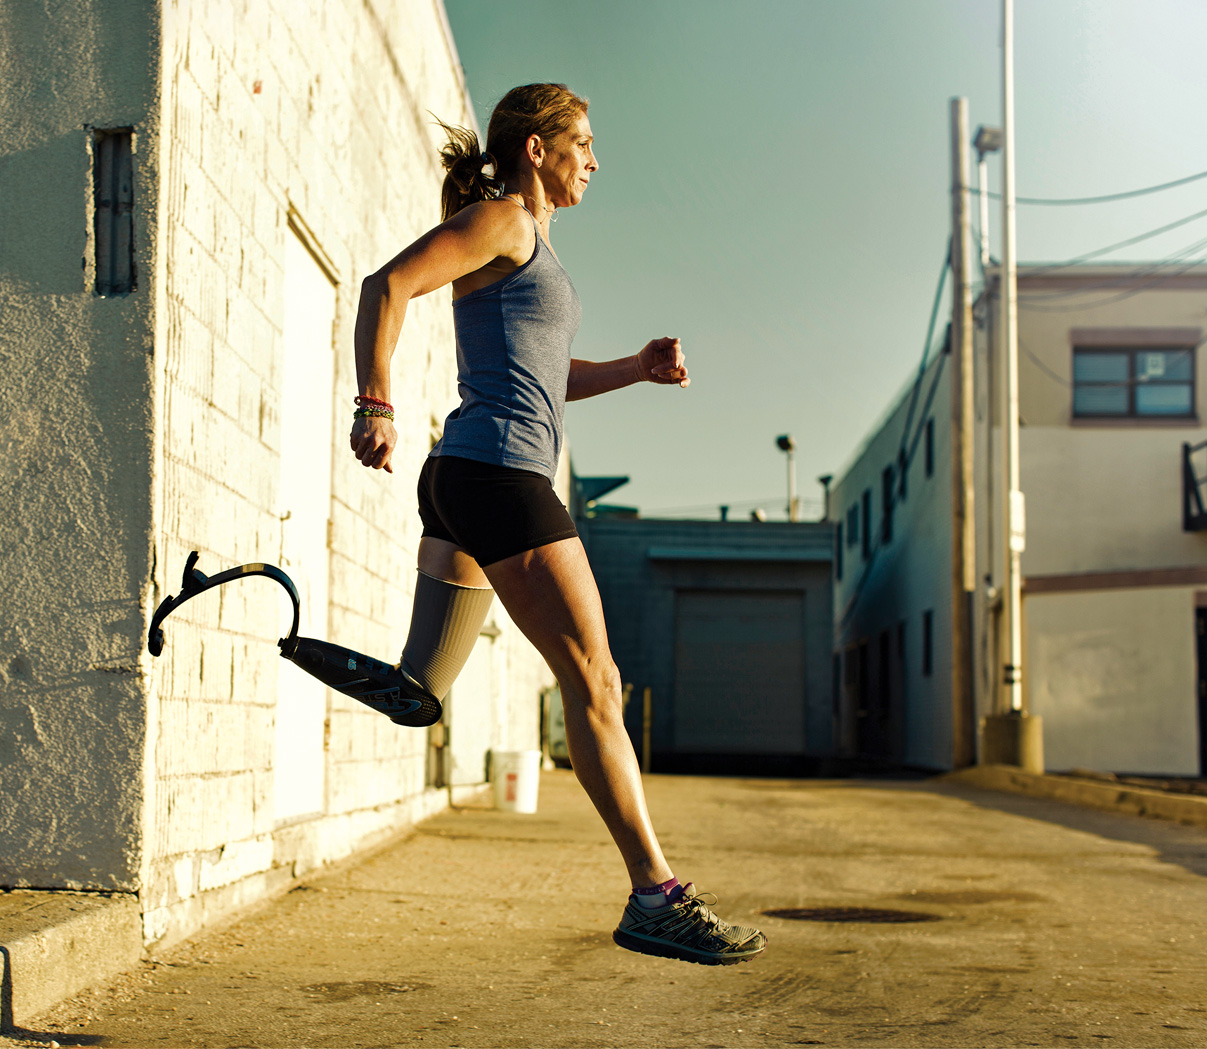
\includegraphics[width=1.0\linewidth]{chap3/3_0}
	% 加星号(*)表示不加编号
	\caption*{ \label{fig:3_0}}
\end{figure}

看过《侏罗纪公园》的人可能都记得那个标志性的场景:
一辆吉普车试图超越一只追赶的霸王龙。
有趣的是,这个场景与电影上映时(1993年)古生物学家的普遍看法相符。
当时人们认为霸王龙的奔跑速度可以达到 40 公里/小时,一些科学家甚至认为它的速度甚至可能更快。
以这样的速度,它在土路上完全可以超过一辆吉普车。


然而,自 2002 年约翰$\cdot$哈钦森(John Hutchinson)开创性论文以来,近期的生物力学研究表明,霸王龙可能根本无法奔跑。
即使它能跑,也可能无法达到 40 公里/小时的速度。
哈钦森通过模拟霸王龙,证明要达到这样的速度,其 86\% 的体重必须由腿部肌肉构成,留给其庞大的尾巴、头部和躯干的空间非常有限。
为了产生足够大的地面反作用力,它需要将如此大的质量分配给腿部肌肉,而这种反作用力在奔跑时通常超过体重的两倍。


对恐龙、大象和袋鼠等动物的研究有助于我们理清对人类跑步的理解:
是什么驱动着从步行到跑步的转变,又是什么限制了跑步速度。
地面反作用力的测量揭示了为什么跑步时比步行时更容易受伤,以及如何设计跑道来降低受伤率并提高速度。


在本章中,我们将使用简单的力学模型来探讨这些问题。
这些模型包含弹簧,用于表示肌肉和肌腱的弹性特性,并揭示弹性能量的储存和释放如何提高跑步效率。
首先,我们定义跑步步态周期,并研究其中涉及的力和弹性机制。
然后,我们将探索一些原理,帮助你设计跑道、跑鞋和假肢,从而实现快速高效的跑步。
我们还会研究从步行过渡到跑步时步态和能量消耗的变化。


\section{跑步步态周期}

跑步步态周期由单腿支撑和腾空交替的阶段组成(图~\ref{fig:3_1})。
与步行类似,一个跑步步态周期由同一条腿连续 2 次触地事件定义,其中对侧腿的触地发生在半程。
每条腿都有一个\textit{支撑期}(脚与地面接触)和一个\textit{摆动期}(脚离地)。
支撑期始于脚触地,结束于脚趾离地,在人类跑步过程中约占步态周期的 30\% 到 45\%,但在高速冲刺过程中可能只占 25\% 或更少。
回想一下,步行时支撑期的持续时间会随着步行速度的增加而缩短。
因此,随着步行速度的增加,双腿支撑的持续时间会缩短。
如果进一步提高速度,每条腿对应的支撑期最终将持续不到步态周期的一半,从而进入腾空期。


\begin{figure}[!htb]
	\centering
	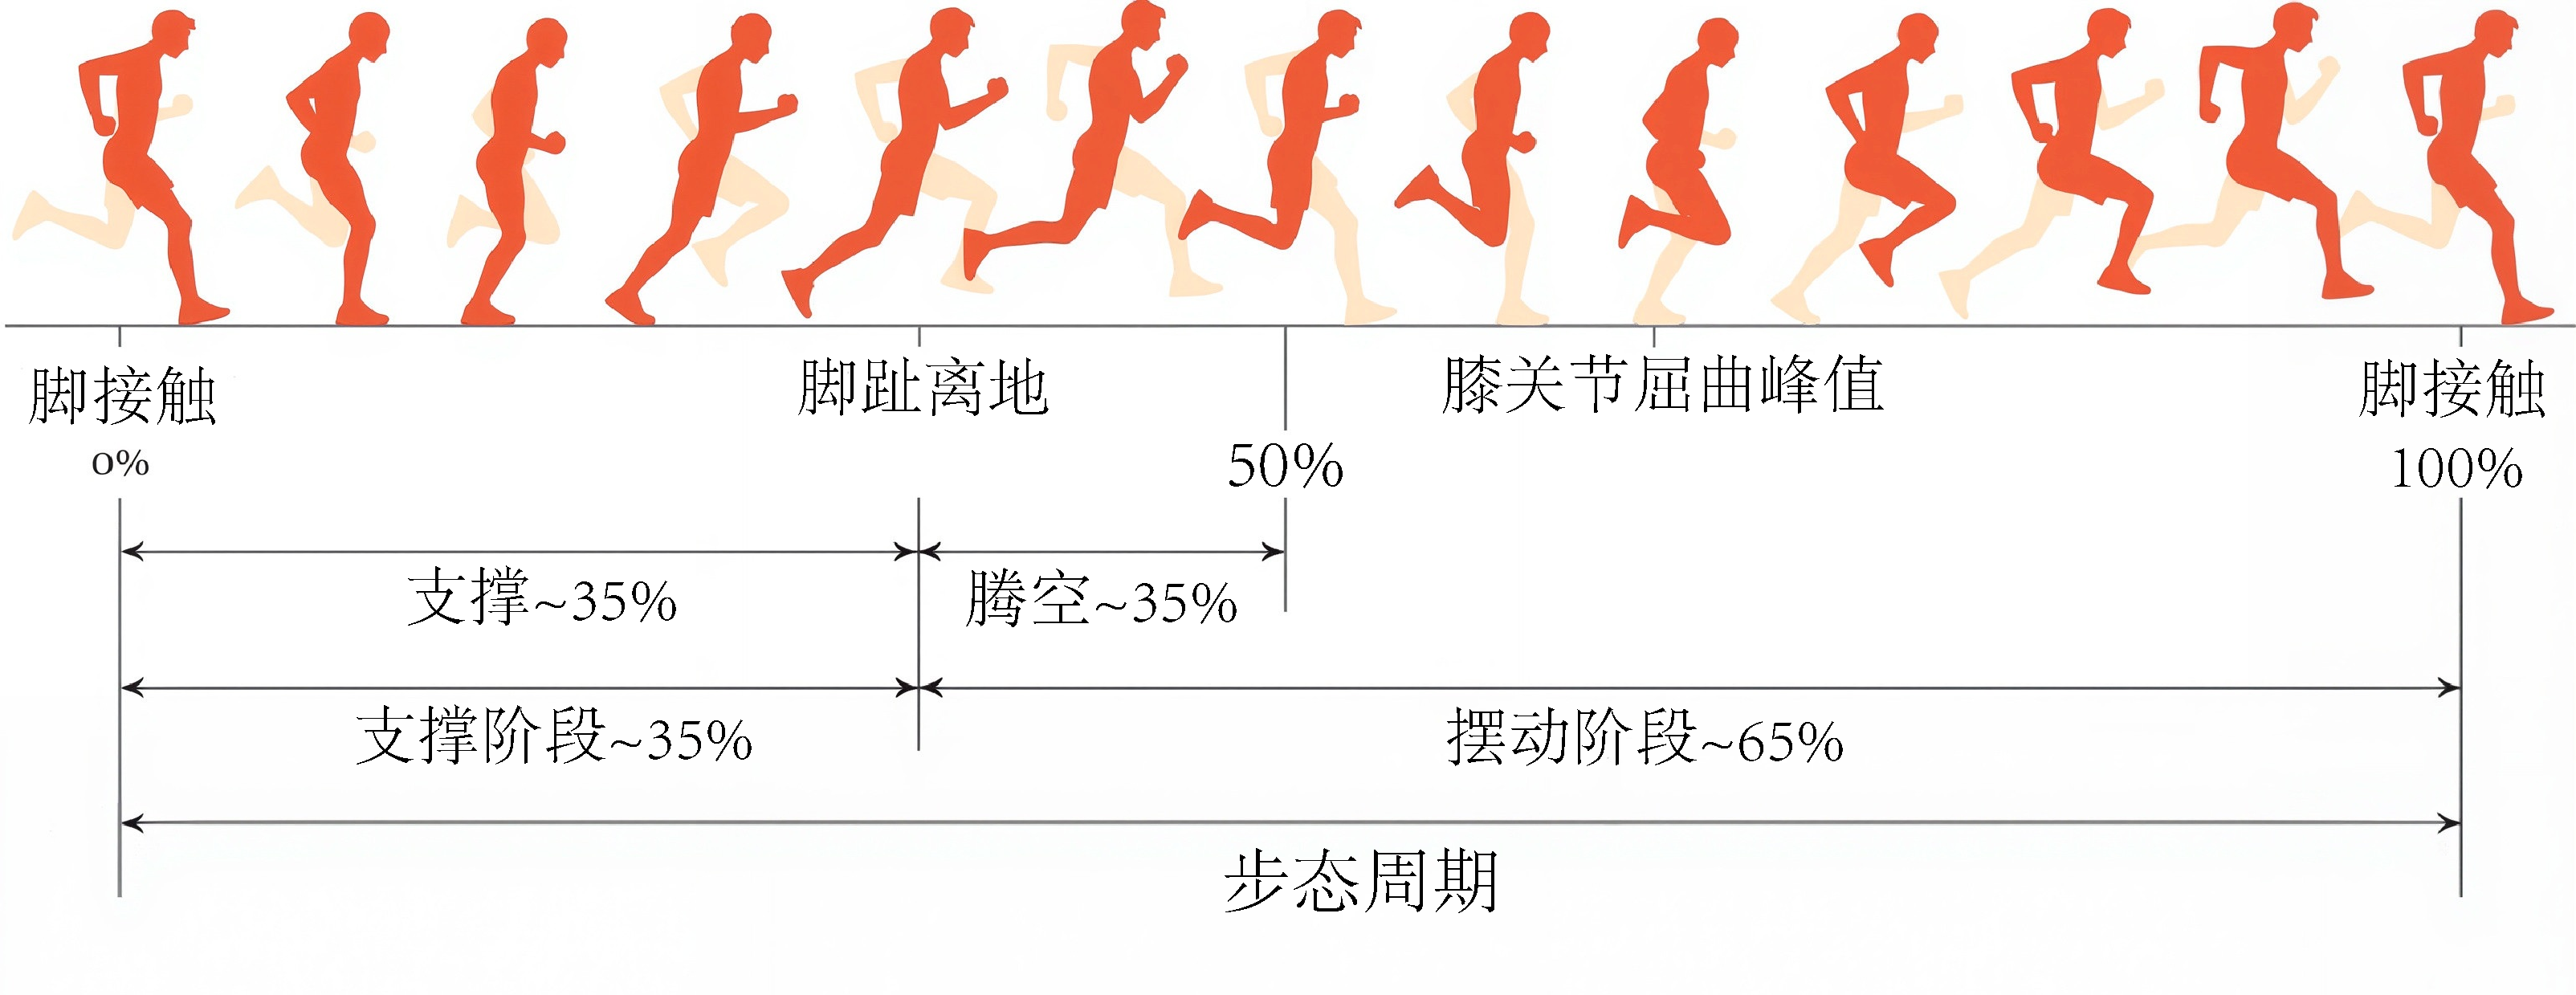
\includegraphics[width=1.0\linewidth]{chap3/3_1}
	\caption{跑步步态周期及其组成事件(例如,脚部触地)和阶段(例如,支撑)。
		站立和摆动的时间百分比会随着跑步速度和风格而变化。 \label{fig:3_1}}
\end{figure}

腾空阶段的存在是我们区分行走和跑步的一个方式。
事实上,人们很容易相信它是跑步的特征,不仅对人类如此,对其他动物也是如此。
然而,我们很快就会看到,当我们从行走步态转换为跑步步态时,会发生另一种质的变化,从生物力学的角度来看,这一点更为重要。


用于量化跑步步态周期的指标与用于步行的指标类似。
步长是两个连续足迹之间沿行进线的距离。
连续两步所走的距离,或一个步态周期所走过的距离,称为步长。
足部接触事件发生的速率(相当于步长持续时间的倒数)称为步频;
迈步的速率称为步频。
跑步速度可以用步长与步频的乘积来计算,
或者,也可以用步长与步频的乘积来计算:

\begin{equation}
	\text{速度(米/秒)} = \text{步长(米/步)} \times \text{节律(步/秒)} \label{eq:3_1}
\end{equation}

中等跑步速度为 4 米/秒。
在此速度下,支撑期约占步态周期的 35\% 至 40\%,典型的步频为 180 步/分钟,典型的步长约为 1.3 至 1.4 米:

\begin{equation}
	\text{步长} = \frac{4.0 \text{米}}{1 \text{秒}}
				 \times \frac{60 \text{秒}}{1 \text{分钟}}
				 \times \frac{1 \text{分钟}}{180 \text{步}}
				 = 1.33 \text{米/秒}
				 \label{eq:3_2}
\end{equation}

当然,这些数量会随着腿长、跑步风格、鞋类和其他因素而变化。


\section{地面反作用力}

正如我们在第~\ref{chap:chap2}~章中所看到的,我们可以通过测量地面反作用力随时间的变化来深入了解步态的动力学和能量学。
跑步时,地面反作用力的垂直分量在足部触地后迅速上升,并在步态周期的约15\%到20\%处达到最大值(图~\ref{fig:3_2})。
在中等速度跑步时,垂直地面反作用力在约 2 倍体重时达到峰值。
水平地面反作用力在站立的前半段指向后方,使重心减速,之后指向前方。

\begin{figure}[!htb]
	\centering
	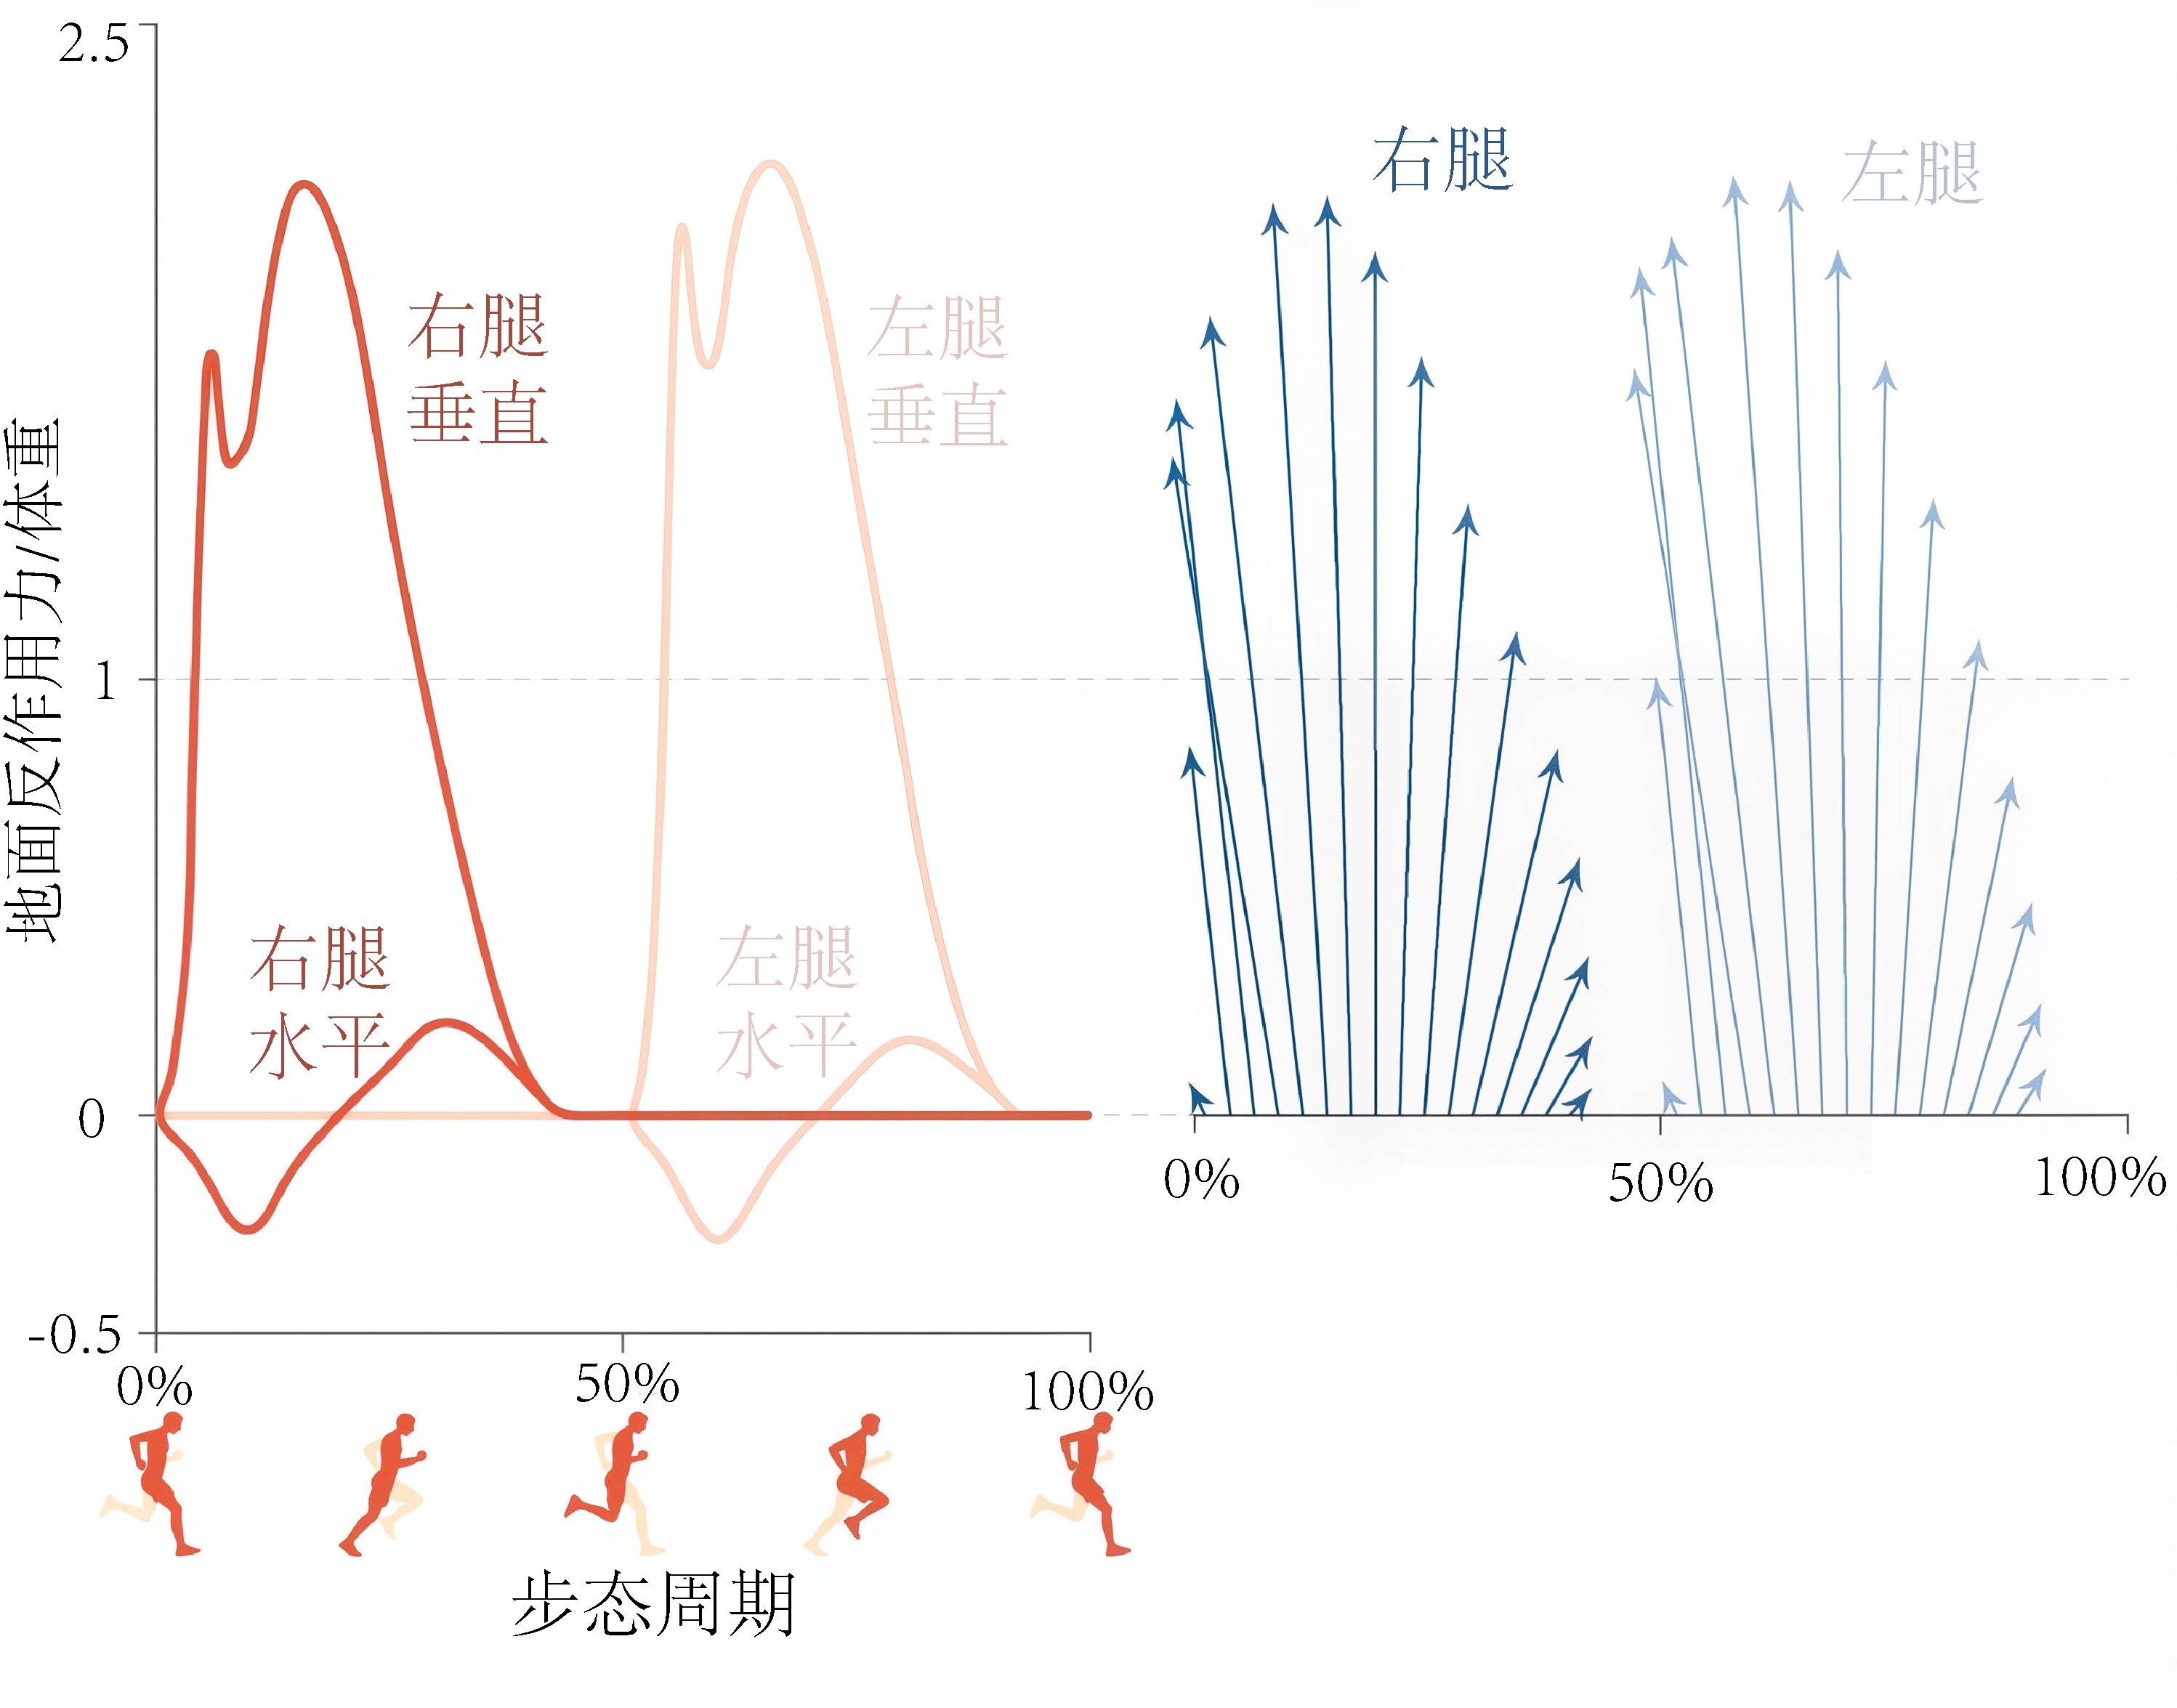
\includegraphics[width=1.0\linewidth]{chap3/3_2}
	\caption{跑步时足跟着地时代表性的地面反作用力。
		图中显示了步态周期内的垂直和水平(前后)分量(左)以及总矢量示意图(右)。
		垂直地面反作用力在足跟着地时出现一个急剧的峰值\cite{yong2020foot}。 \label{fig:3_2}}
\end{figure}

图~\ref{fig:3_2}~显示了后脚掌着地的跑步者(即用脚跟着地的跑步者)身上特有的双峰垂直地面反作用力。
虽然行走时的地面反作用力也有两个峰值,但跑步时第一个峰值较短,是由于脚跟着地产生的。
某些跑步者,尤其是那些从小就赤脚跑步的跑步者,会用前脚掌着地。
对于这些跑步者来说,垂直地面反作用力上升得更平缓,并且只有一个峰值(图~\ref{fig:3_3})。
有人认为这种跑步方式更“自然”,可以防止与冲击相关的伤害,但后续研究对这一结论提出了质疑。
从小就用后脚掌着地的跑步者如果改为用前脚掌着地,尤其是在没有经过适当训练的情况下,可能会有受伤的风险。

\begin{figure}[!htb]
	\centering
	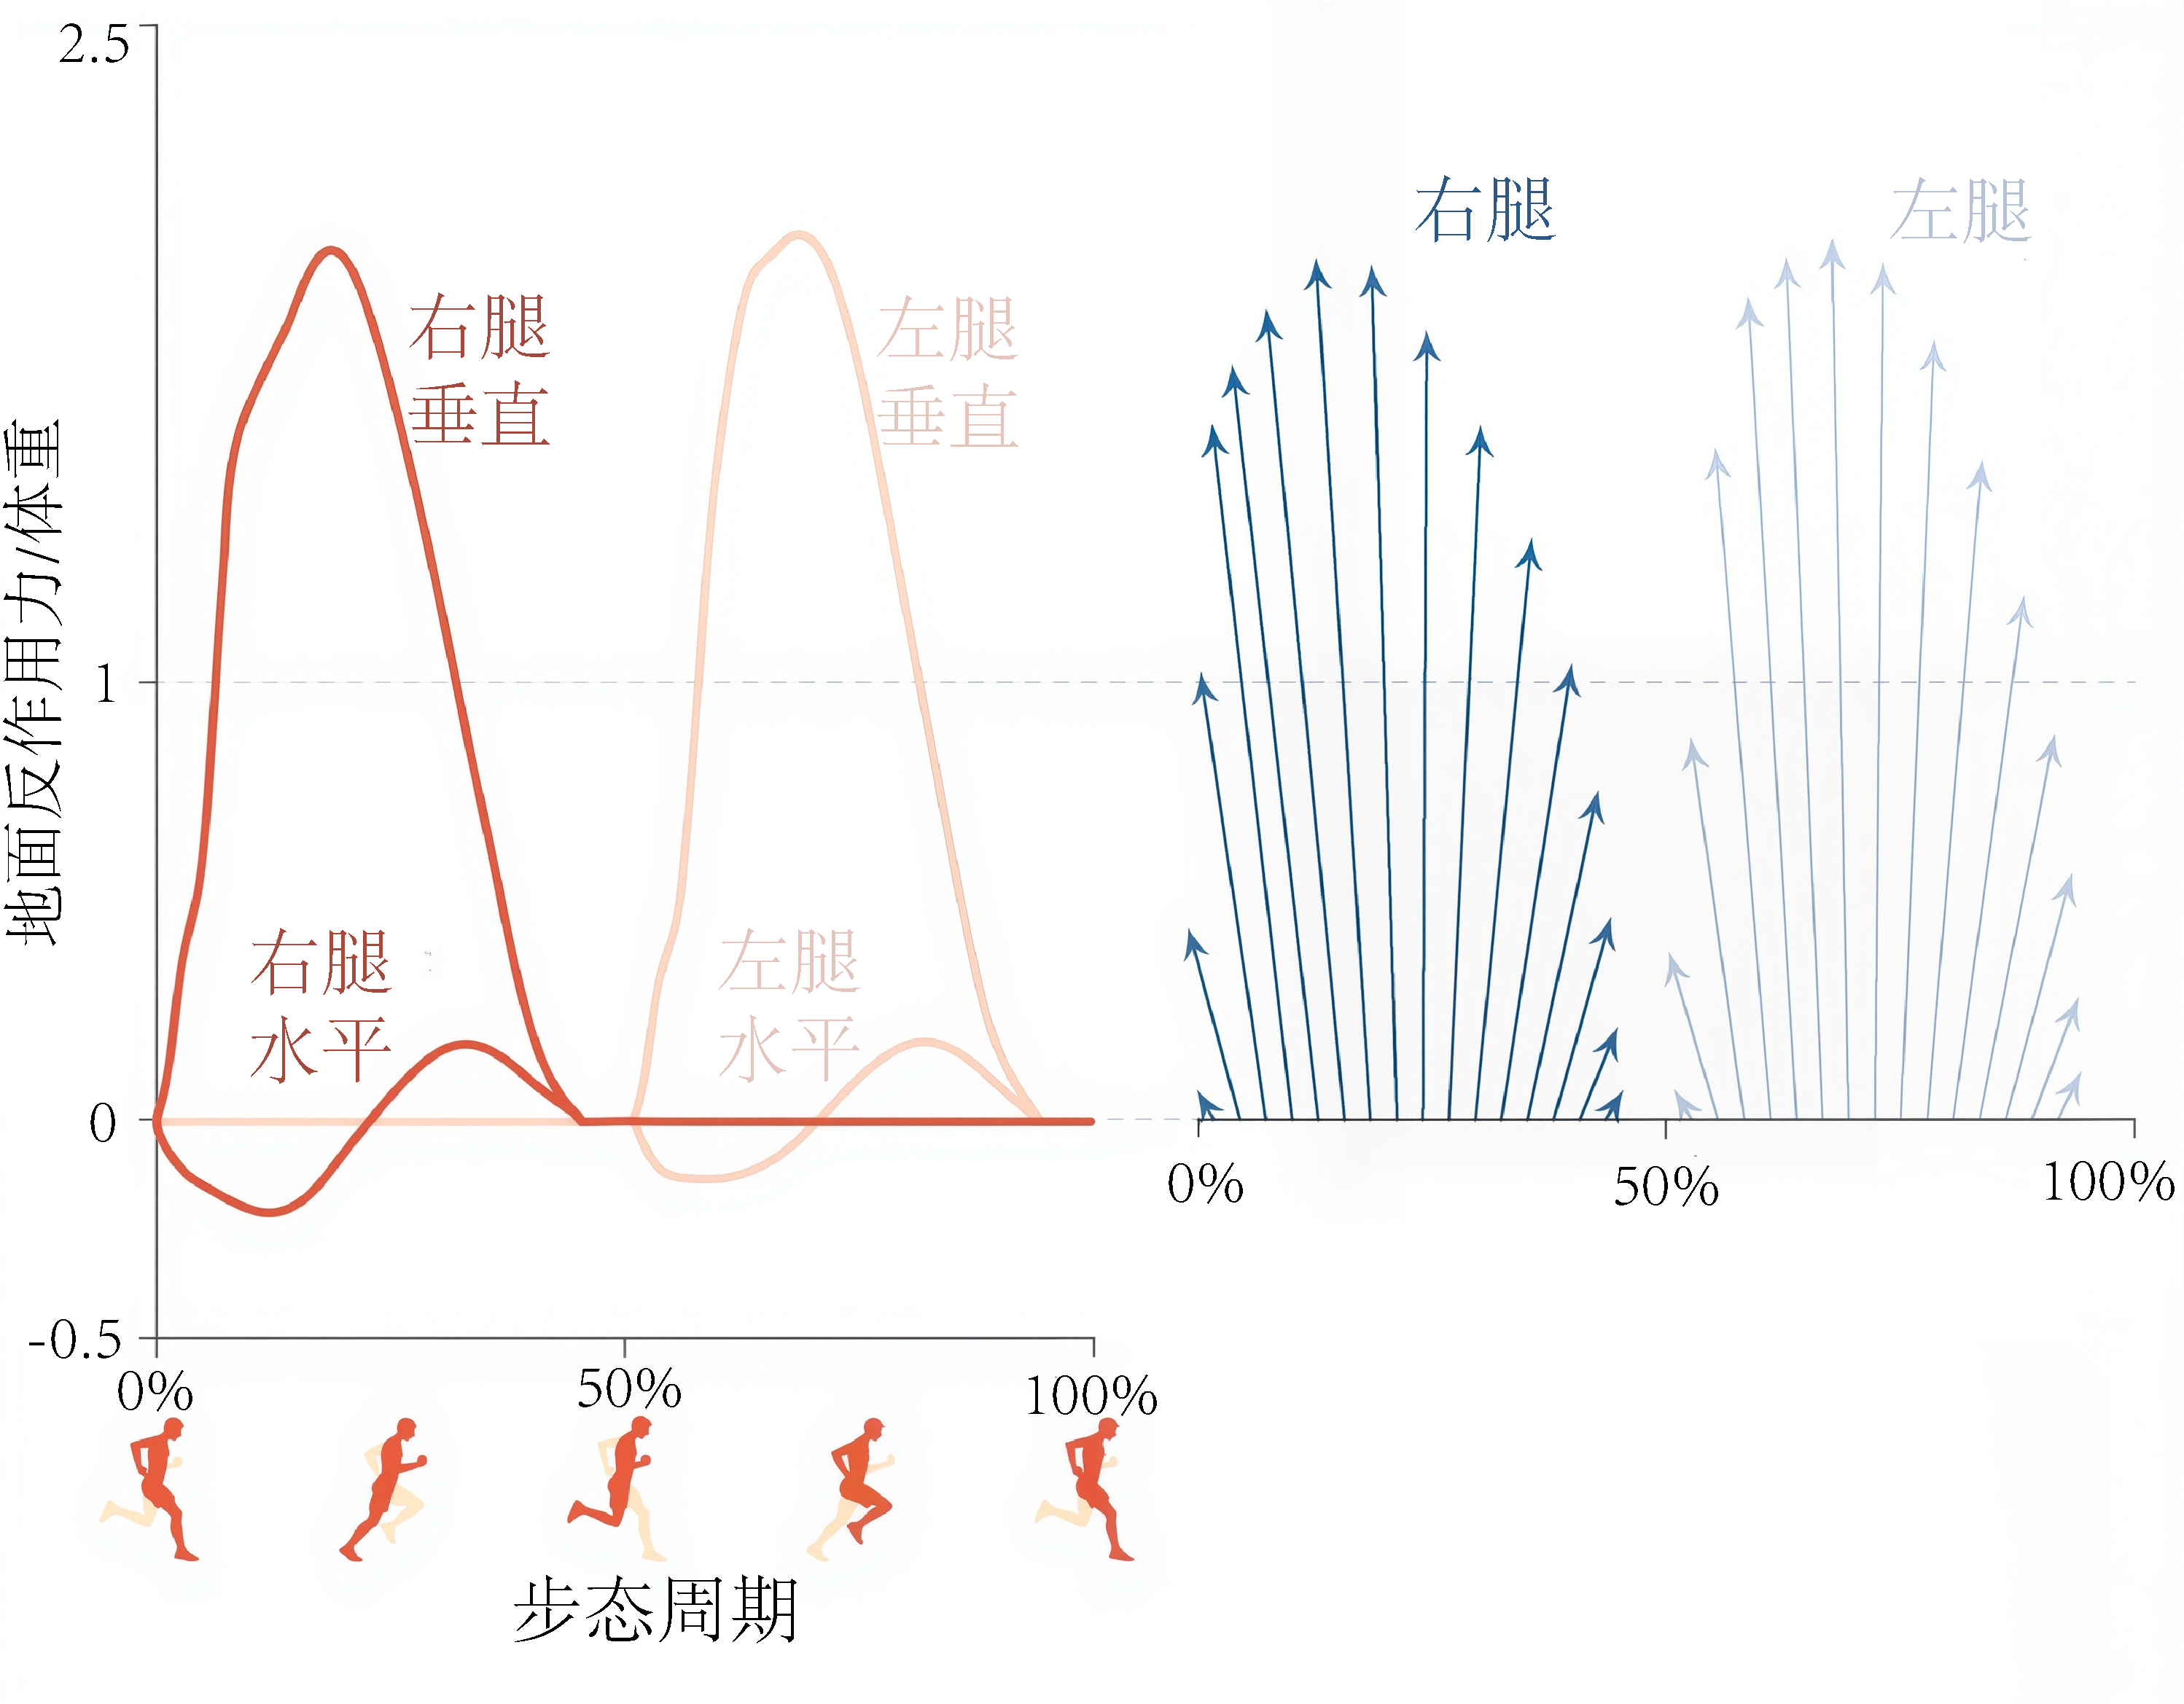
\includegraphics[width=1.0\linewidth]{chap3/3_3}
	\caption{前脚掌落地时,跑步过程中地面反作用力的代表性数据,与图~\ref{fig:3_2}~中的受试者相同。
		垂直地面反作用力没有后脚掌落地时出现的尖峰,这可能有助于降低受伤风险\cite{yong2020foot}。 \label{fig:3_3}}
\end{figure}


跑步时,前向动能和重力势能可以用公式~\ref{eq:2_3}~和公式~\ref{eq:2_4}~计算(图~\ref{fig:3_4})。
在跑步的腾空阶段(忽略空气阻力),前向速度和前向动能最大,且近似恒定。
重心在腾空过程中也最高,因此重力势能也最高。
因此,与行走不同,前向动能和重力势能大约同时达到最大值。
同样,前向动能和重力势能都在站立中期达到最小值,也就是说,当重心最低时,前向速度大约最小。

\begin{figure}[!htb]
	\centering
	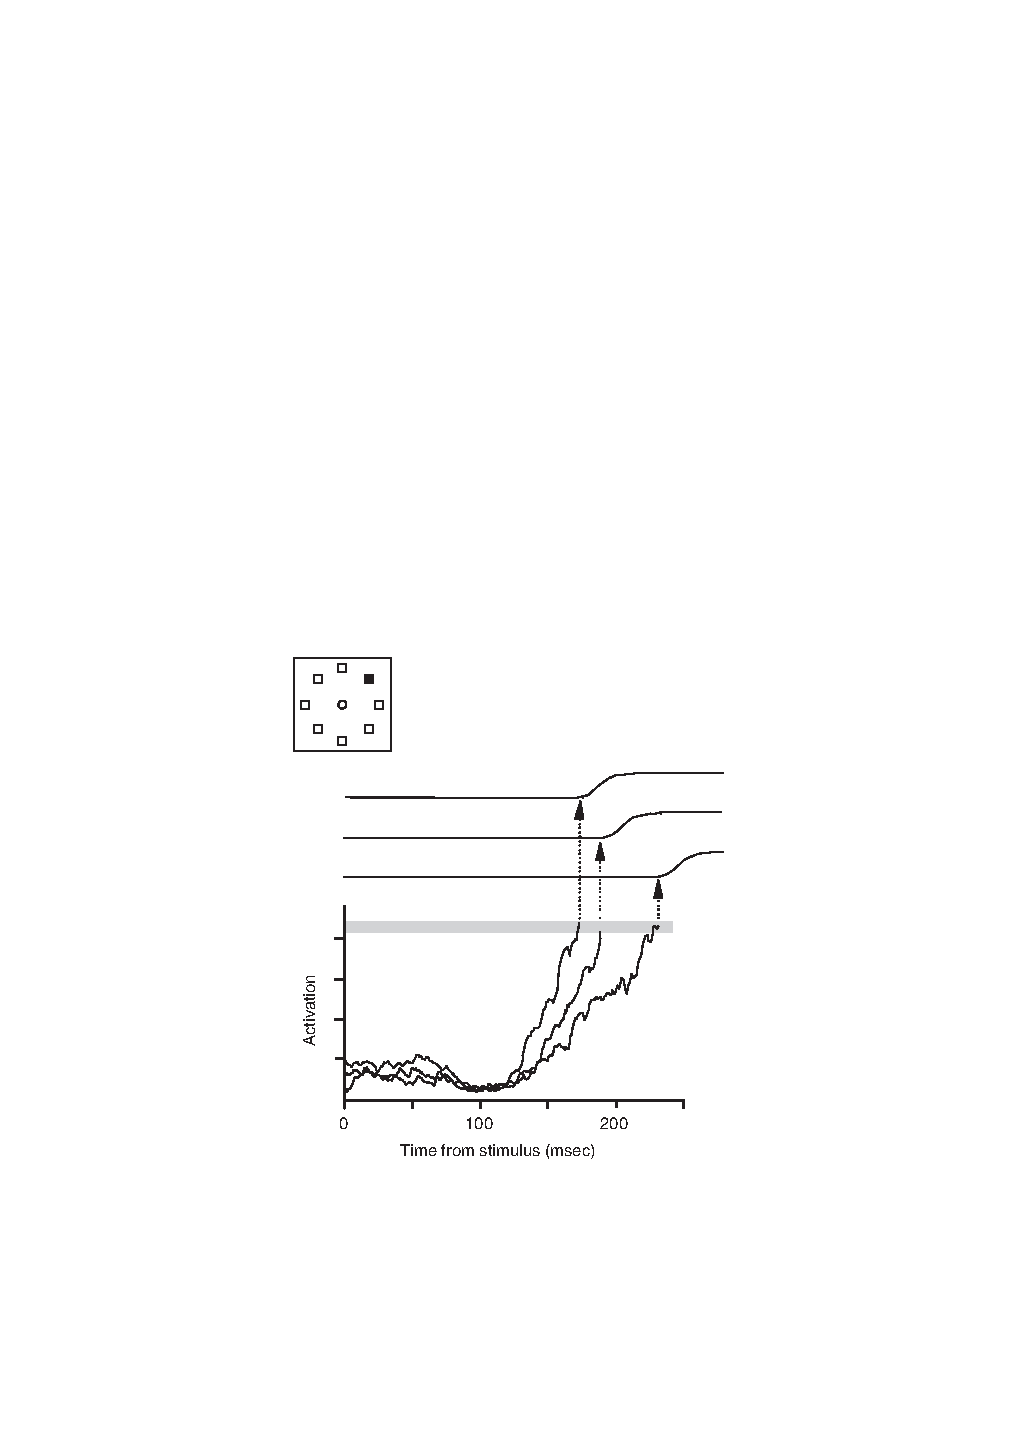
\includegraphics[width=1.0\linewidth]{chap3/3_4}
	\caption{奔跑过程中的代表性重力势能和前向动能。
		飞行过程中,前向动能保持不变\cite{yong2014differences}。 \label{fig:3_4}}
\end{figure}


我们想强调步行和跑步之间的一个根本区别:
在跑步时,我们并非从向前的动能和重力势能的交换中获益,而是在肌肉和肌腱的伸展和回弹过程中储存和释放弹性势能。
这一观察结果暗示了一种如图~\ref{fig:3_5}~所示的跑步模型。
在该模型中,质量在站立中期达到最低点,此时质心的向前速度也最小,这与我们在实验数据中发现的情况相似。
我们腿部如同弹簧般的运动使跑步成为一种能量高效的步态。

\begin{figure}[!htb]
	\centering
	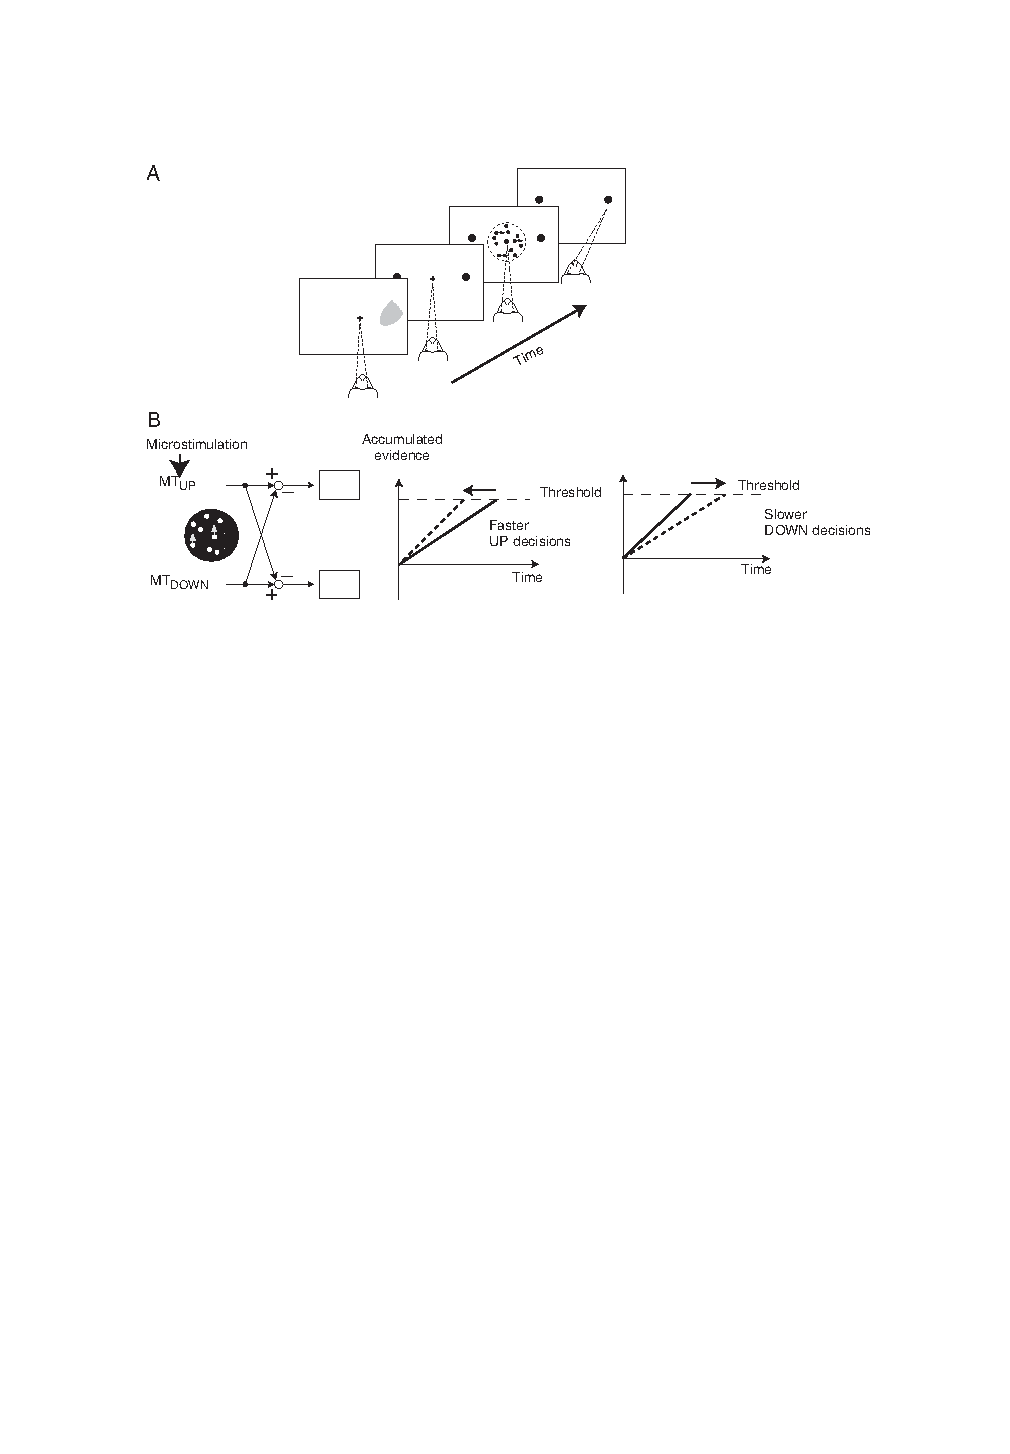
\includegraphics[width=1.0\linewidth]{chap3/3_5}
	\caption{跑步的站立阶段(左)及其质量弹簧模型(右)。
		在该模型中,身体的质量被集中到一个点质量上,该点质量位于代表腿部的无质量线性弹簧的顶部。
		弹簧压缩,质量在站立中期达到最低点,此时质量的前进速度也最低。 \label{fig:3_5}}
\end{figure}


正如我们在第~\ref{chap:chap2}~章中看到的,大象即使在尽可能快地移动时也没有飞行阶段。
因此,你可能会认为大象不会跑。
但事实上,它们似乎有一种“格劳乔式行走”,膝盖弯曲,重力势能和向前动能的波动同步。
从生物力学的角度来看,这种同步意味着大象在某种意义上是在奔跑。
就像人类一样,这些厚皮动物利用腿作为弹簧来储存能量,如图~\ref{fig:3_5}~所示。
大象很可能进化出这种不腾空而起的“奔跑”方式,以适应它们巨大的体型。
正如我们将在本书后面看到的,肌肉力量与肌肉的横截面积(长度的平方)成正比,而体重与体积(长度的立方)成正比。
因此,体型巨大的动物与体型较小的动物相比,体型较大的动物具有较低的力量重量比。
这个原理解释了为什么像松鼠这样的小动物可以产生很大的地面反作用力并跳跃几个身长的距离,而大象和霸王龙(它们的大小大致相同)却无法产生足以让它们瞬间飞翔的地面反作用力。



\section{跳跃和跑步中的弹性机制}

另一种能够让我们了解跑步过程中弹性能量储存的动物是袋鼠。
袋鼠的奔跑并非传统意义上的奔跑;
我们通常将它们的动作描述为跳跃。
然而,从生物力学的角度来看,它们使用的机制与人类跑步时类似。


20世纪70年代初,特伦斯$\cdot$道森和理查德$\cdot$泰勒训练袋鼠佩戴面罩,在跑步机上以1至22公里/小时的速度跳跃——这项实验无疑需要高超的动物操控技巧。
面罩让研究人员能够测量动物的代谢能量消耗,而这正是泰勒当时研究的主题。
他针对袋鼠和其他​​动物进行的大量实验,让生物学家们注意到能量消耗是影响动物行为的关键因素。


道森和泰勒发现,低速时,袋鼠不会跳跃,而是采用五足步态,即用尾巴作为与地面的第五个接触点(图~\ref{fig:3_6})。
这种运动方式看起来很笨拙,而且能量效率低下。
事实上,他们发现,当袋鼠以更高的速度(从 1 到 6 公里/小时;图~\ref{fig:3_7}A)蹒跚向前时,能量消耗急剧增加。
五足步态下速度的提升主要通过增加步频实现(图~\ref{fig:3_7}D)。
当速度达到约 6-7 公里/小时时,袋鼠会过渡到跳跃。
图~\ref{fig:3_7}A~中一个引人注目的特征是,当袋鼠的速度超过 7 公里/小时时,运送成本略有下降。
如图~\ref{fig:3_7}C~和 D 所示,在跳跃阶段,它们主要通过增加步幅来提高速度。
步频几乎保持不变。这一结果与袋鼠的质量弹簧模型(类似于图~\ref{fig:3_5})一致,因为弹簧质量的固有频率不会随着其运动幅度的变化而变化。
Dawson和Taylor指出,袋鼠的跟腱非常适合储存和释放弹性能量,并认为这种机制使跳跃更加高效,并使其能够高速跳跃。


大约在这个时候,泰勒在意大利乔瓦尼$\cdot$卡瓦尼亚的实验室里了解到了测力板,于是他带着他的动物(袋鼠、猴子、狗和火鸡)来到米兰,在卡瓦尼亚当时刚刚发明的实验中试用它们。
最终的研究成果发表于1977年,进一步证明了袋鼠会储存弹性能,并在跳跃过程中释放。
在高达30公里/小时的速度下,氧气消耗约占袋鼠加速重心所需能量的三分之一;
剩余的能量必定是由肌肉和肌腱中的弹性储存提供的。


\begin{figure}[!htb]
	\centering
	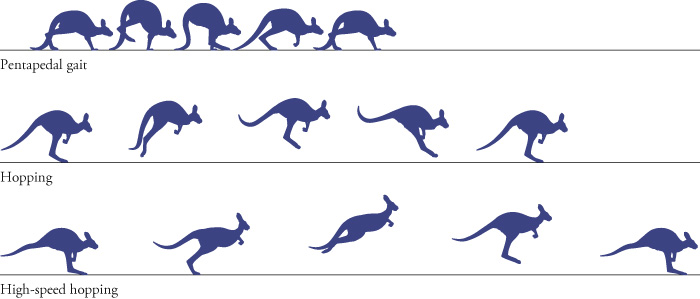
\includegraphics[width=1.0\linewidth]{chap3/3_6}
	\caption{袋鼠的运动方式。
		在慢速运动时,袋鼠采用五足步态(上图),利用尾巴支撑后肢向前移动。
		在高速运动时,袋鼠采用跳跃步态(中图),利用尾巴保持平衡并控制身体倾斜。
		在高速跳跃时(下图),袋鼠的速度可以超过 50 公里/小时\cite{dawson1977kangaroos}。 \label{fig:3_6}}
\end{figure}


\begin{figure}[!htb]
	\centering
	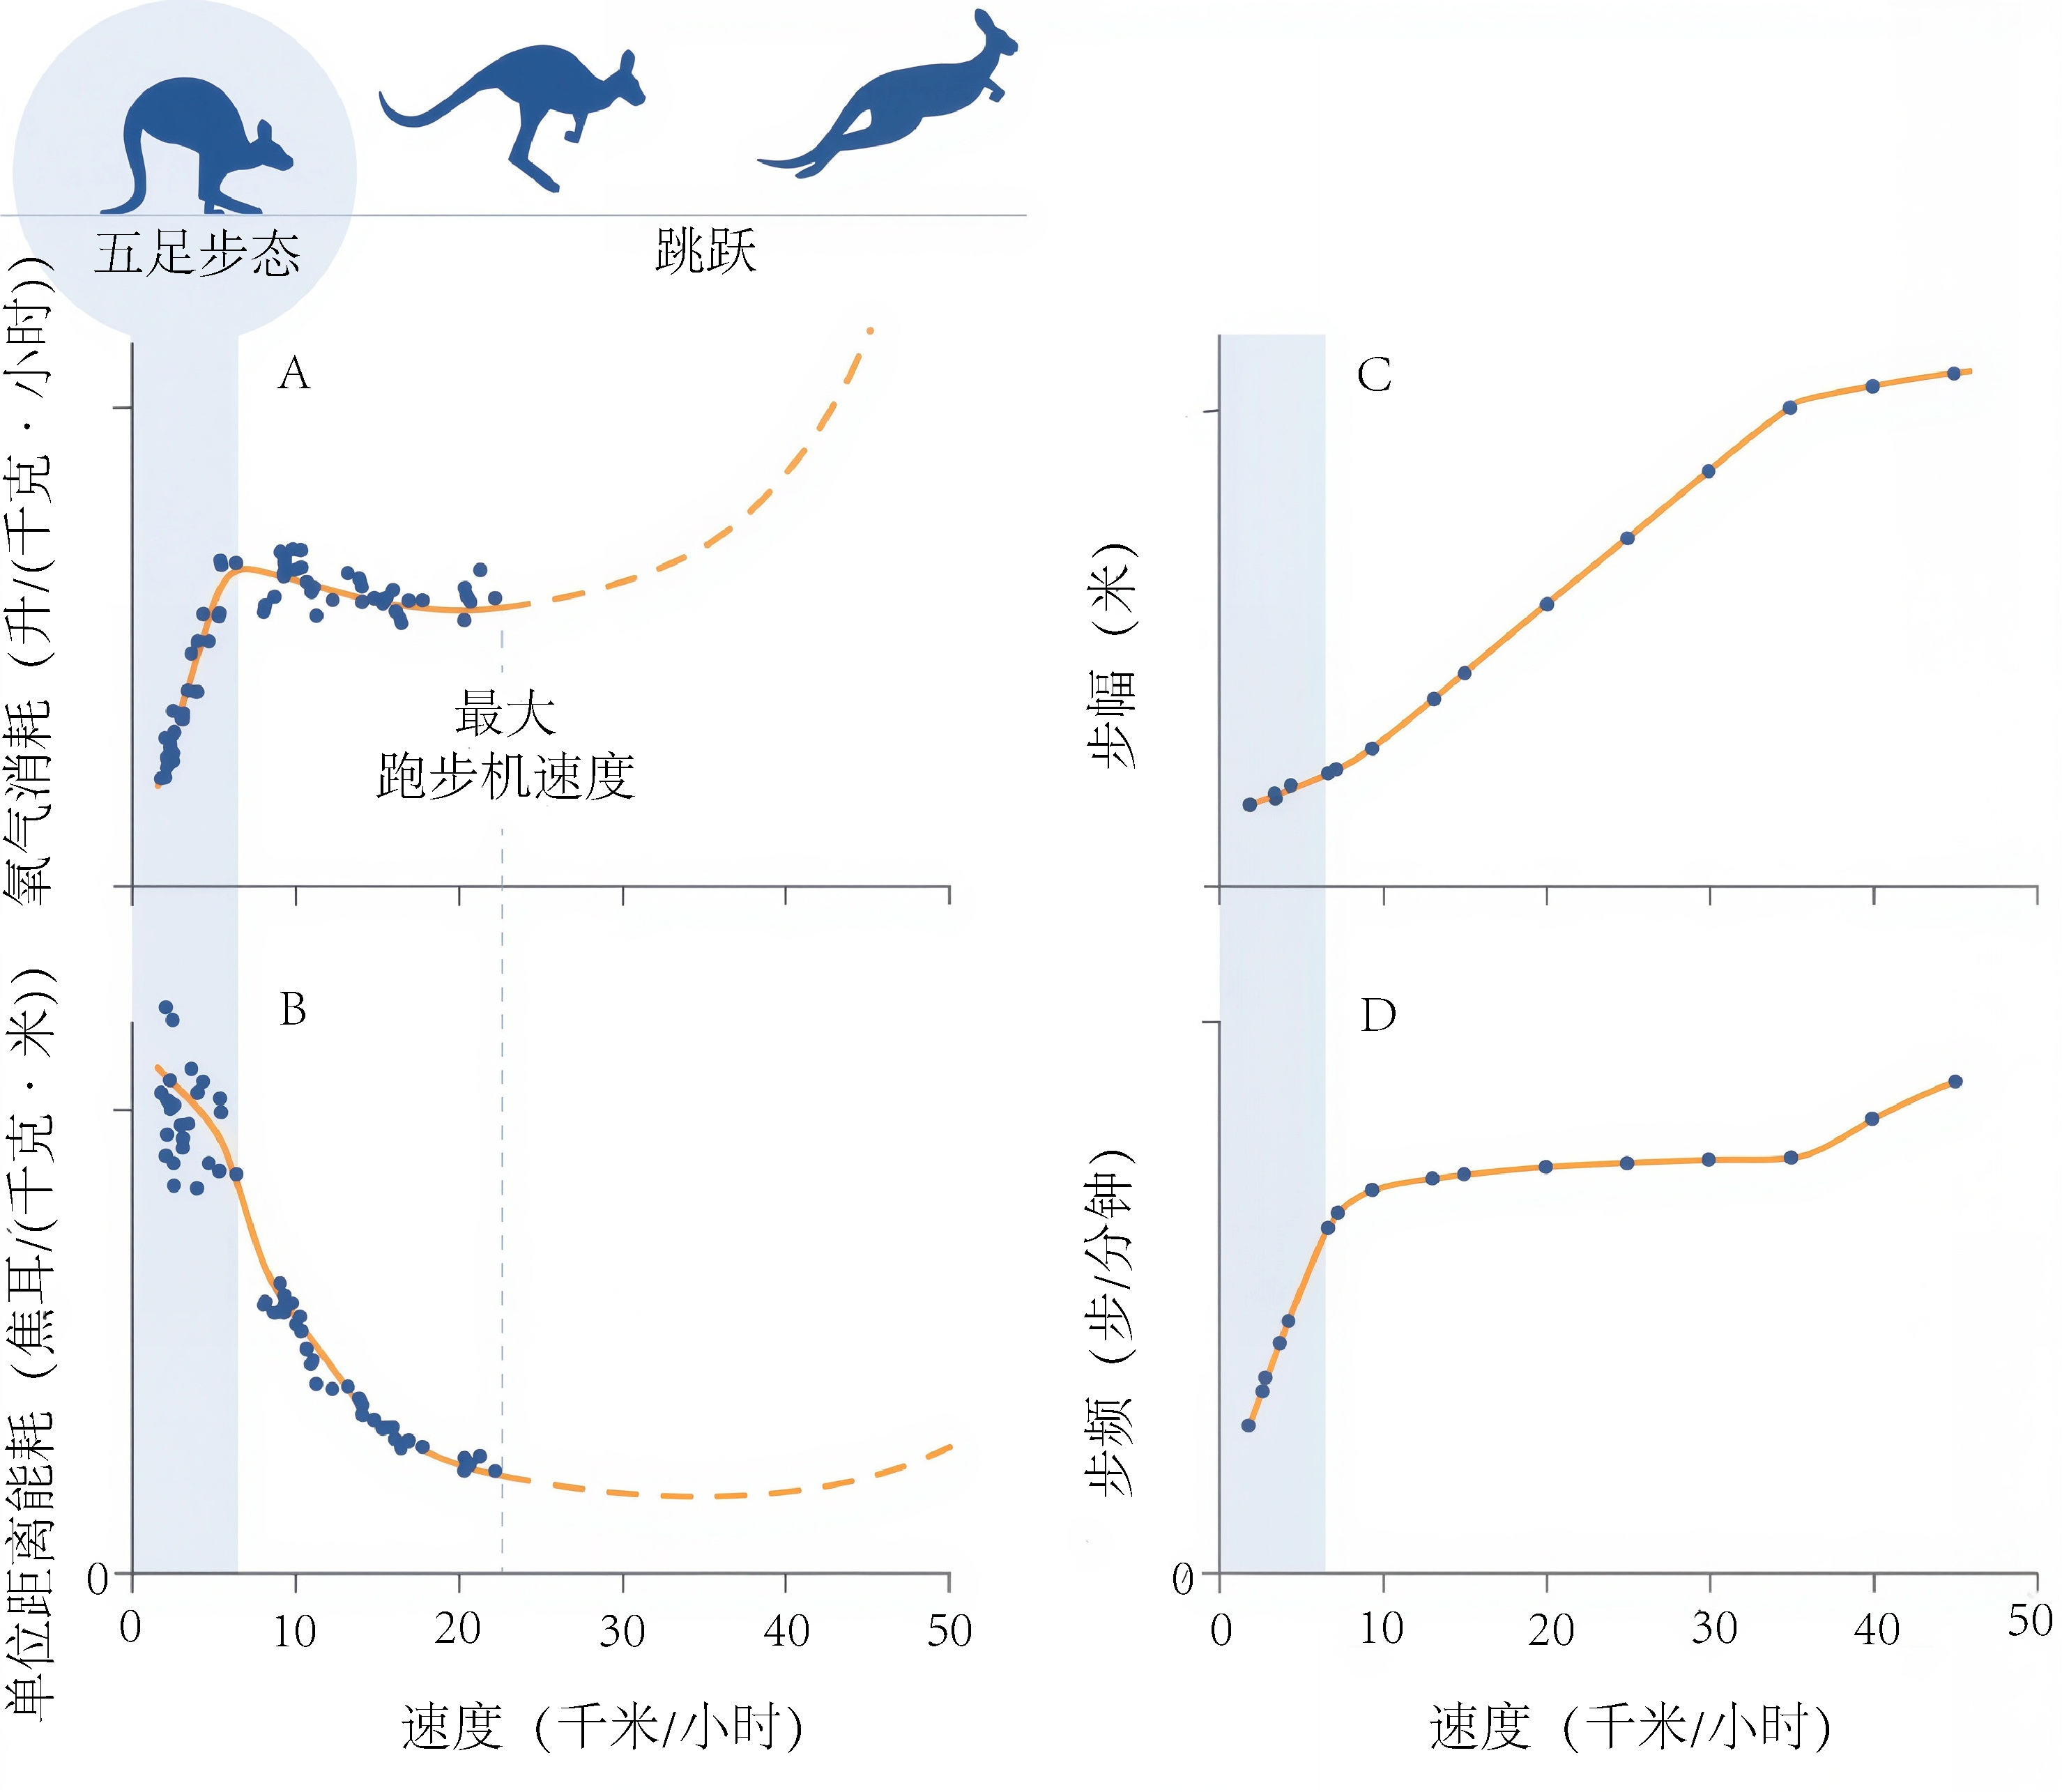
\includegraphics[width=1.0\linewidth]{chap3/3_7}
	\caption{袋鼠运动的能量学。
		在五足步态中,质量标准化的耗氧率随速度增加而增加。
		袋鼠在6-7公里/小时左右过渡到跳跃;
		随后耗氧量随速度增加而下降,直至20公里/小时左右达到最低值。
		Dawson\cite{dawson1977kangaroos}估算了无法在实验室研究的速度下的耗氧量(虚线)。
		在低速跳跃时,步频保持相对恒定,速度主要通过增加步幅来提高\cite{dawson1977kangaroos}。 \label{fig:3_7}}
\end{figure}


\section{跳跃机器人}

许多早期的步行机器人在运动过程中保持静态稳定,向前移动时重心保持在脚部上方。
20世纪80年代,马克$\cdot$雷伯特(Marc Raibert)和他的同事制造了第一批能够在高速运动中保持“动态平衡”的机器人,它们像跑步一样交替进行支撑和飞行。
这些早期的机器人跑步者只有一条腿,依靠运动来保持稳定,只能通过跳跃来保持直立。
这种巧妙的设计将控制问题集中在保持平衡上,同时避免了协调多条腿运动的复杂性。


Raibert 的第一个机器人用一条弹性腿在平面上跳跃(图~\ref{fig:3_8})。
该机器人受到机械约束以防止侧翻,并被拴在一台控制计算机和外部压缩空气及电源上。
腿部在可调节刚度的弹簧(气缸)上弹跳,弹簧为每次跳跃提供所需的能量。
控制器由三个独立组件组成:
第一个组件通过向气缸充气和放气来调节垂直运动,调整腿部刚度;
第二个组件通过在飞行过程中适当定位脚部来保持平衡;
第三个组件通过在站立时在腿和身体之间施加扭矩来稳定身体的姿态(倾斜度)。
腿部摆动是平衡和姿态控制器产生的臀部扭矩的自然结果。
例如,在飞行过程中,平衡控制器必须向前摆动腿部以准备下一个站立阶段。

\begin{figure}[!htb]
	\centering
	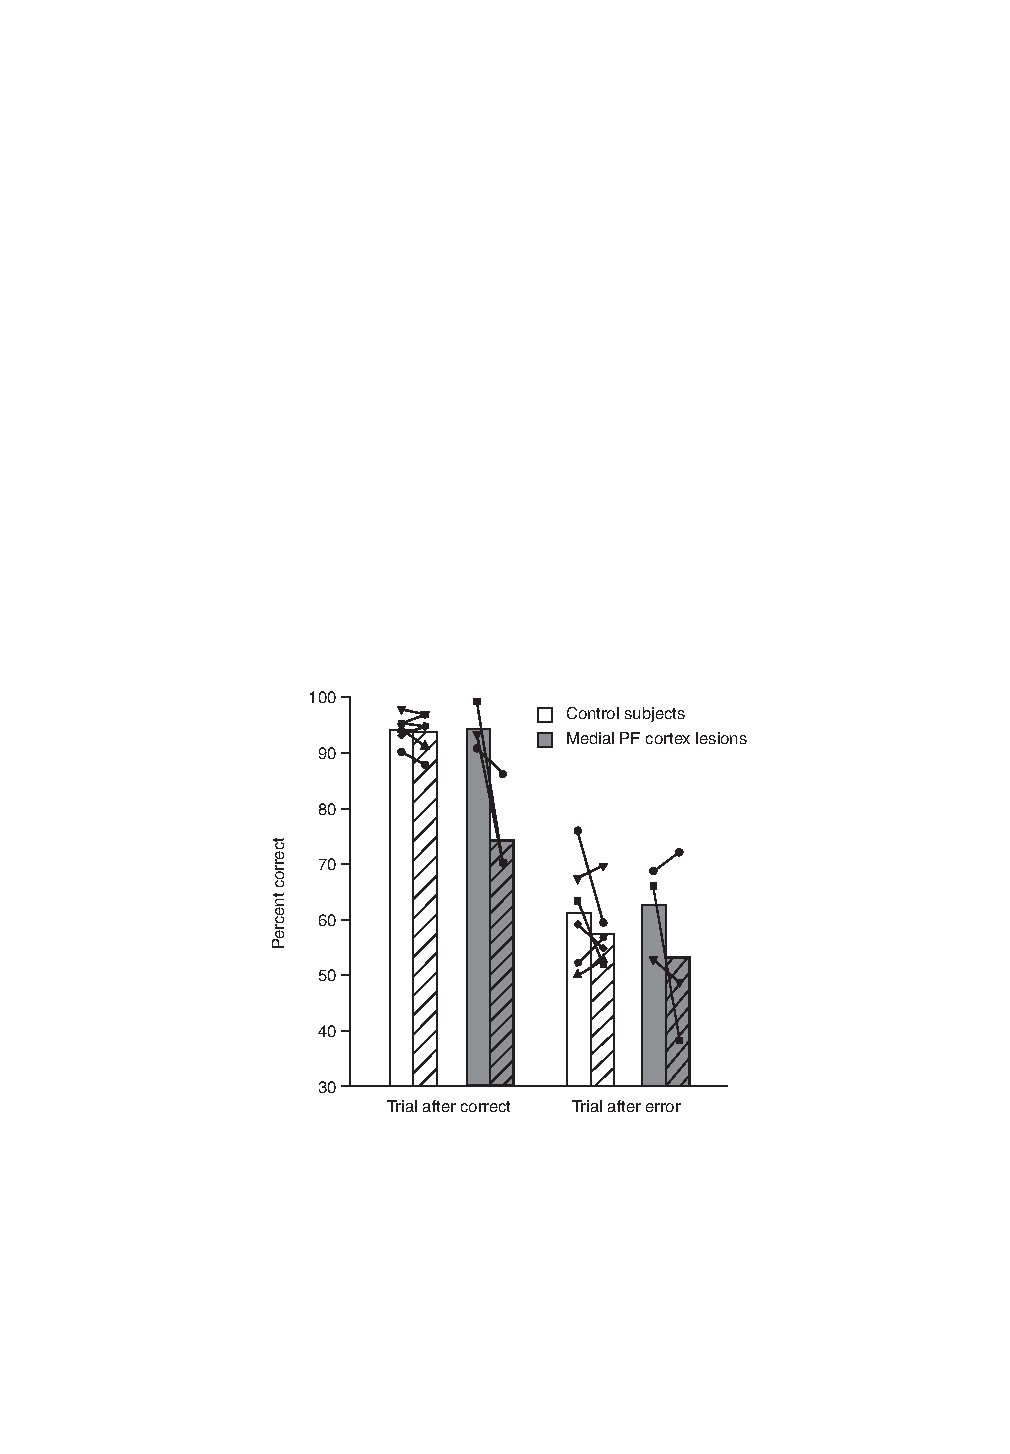
\includegraphics[width=1.0\linewidth]{chap3/3_8}
	\caption{Raibert 平面机器人的运动方式类似于跳跃的袋鼠,尽管它没有尾巴来控制俯仰。
		机载电子设备可以调节臀部角度和腿部刚度,以控制平衡、垂直运动和身体姿态。
		与有袋动物不同,该机器人只能在跳跃时保持平衡\cite{raibert1984machines}。 \label{fig:3_8}}
\end{figure}

同样的三段式控制策略也被用于动态平衡一个类似的3D跳跃机器人\cite{raibert1984machines}。
该机器人同样依靠一条弹性腿弹跳,每次跳跃时储存和释放能量。
然而,与其平面前身不同的是,机器人的躯干不受约束,因此平衡控制器可以调节其俯仰角和滚转角。
该机器人的最高速度可达2.2米/秒(慢跑速度),并且能够从外部扰动中恢复,这由机器人设计师自豪地提供。
Raibert后来于1992年创立了波士顿动力公司,该公司开发了一系列敏捷机器人。
这些机器人已经发展到两条腿和四条腿,但它们仍然基于相同的原理。
在近二十年开发尖端机器人之后,该公司宣布计划于2019年推出其首款商业模型——受犬类启发的SpotMini(图~\ref{fig:3_9})。


\begin{figure}[!htb]
	\centering
	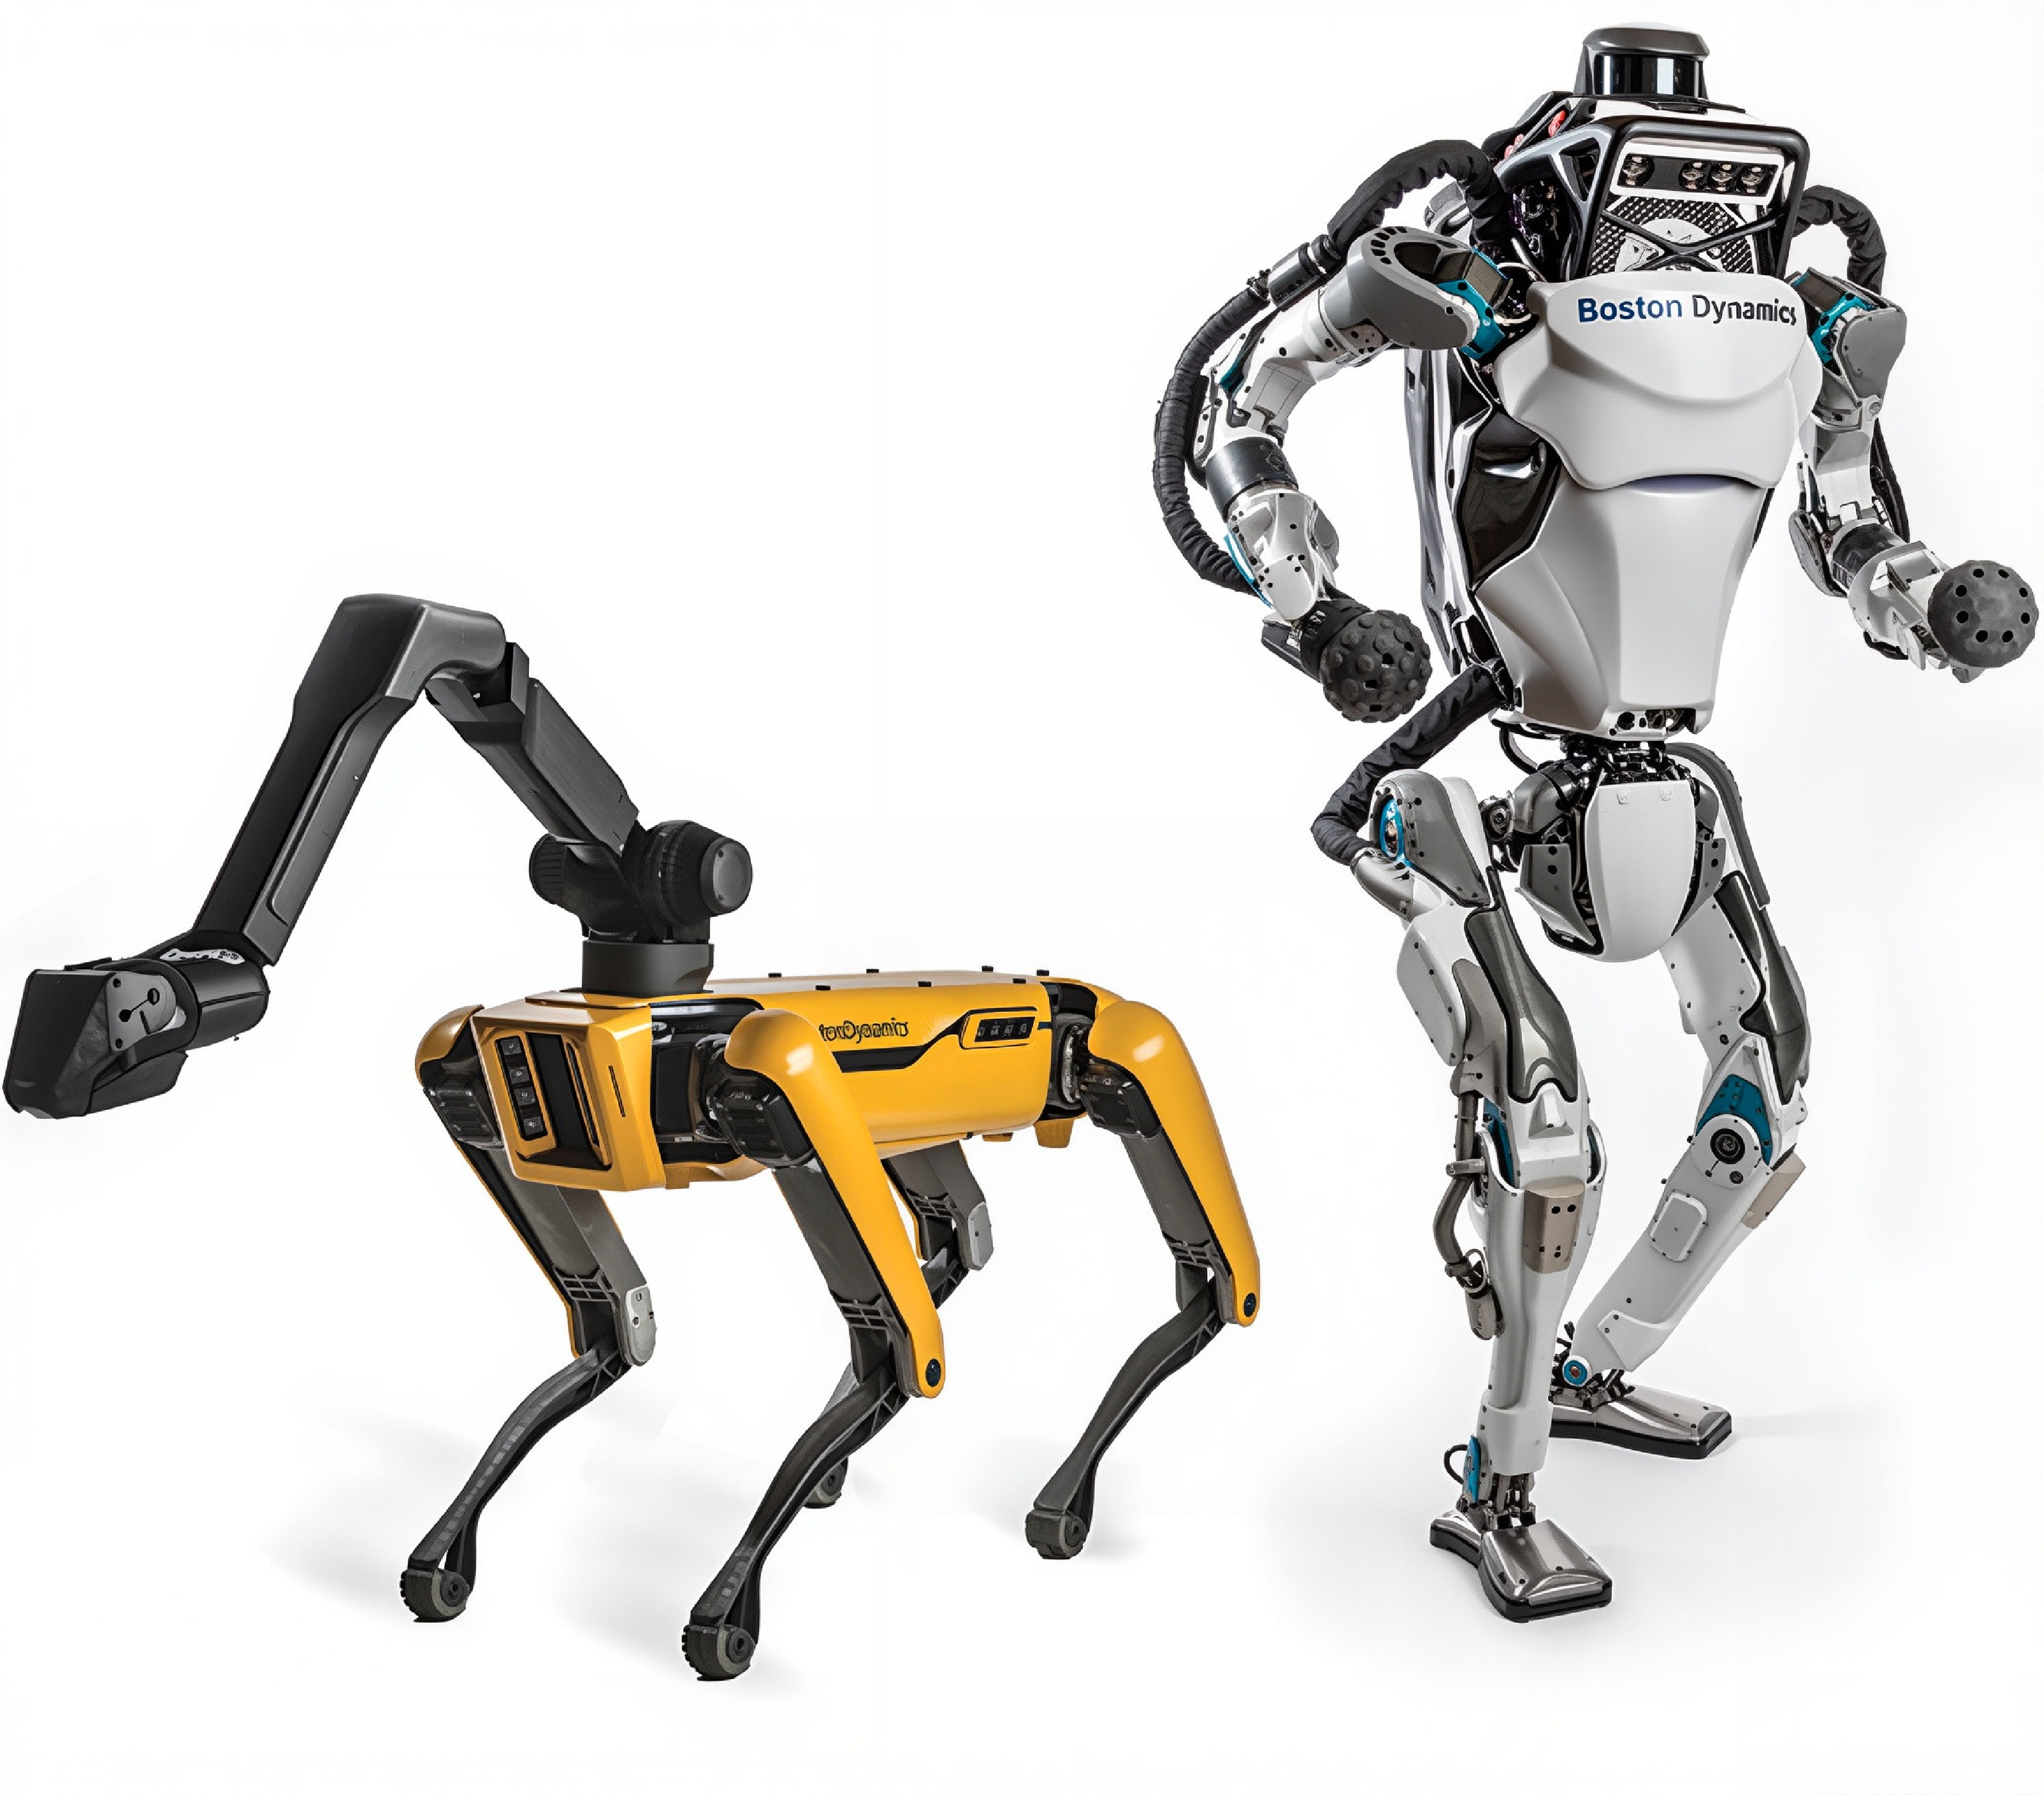
\includegraphics[width=1.0\linewidth]{chap3/3_9}
	\caption{现代跑步机器人的例子。
		Spot 机器人(左)和 Atlas 机器人(右)的照片由波士顿动力公司提供。 \label{fig:3_9}}
\end{figure}


\section{调谐轨迹}

20世纪70年代中期,托马斯$\cdot$麦克马洪接到了一个不寻常的求助电话。
哈佛大学正在修建一条新的室内跑道,承包商与田径教练在弯道坡度应该多大的问题上意见不合\cite{wingerson1983lion}。
在麦克马洪解决了这个问题(支持了田径教练的意见)后,他们又问了他另一个问题:跑道表面应该有多硬?


当时,传统观念认为跑道越硬越好,以尽量减少跑者双脚与地面的接触时间。
但麦克马洪质疑了这种观点。
在他看来,更柔顺(或“弹性”)的跑道可以通过增加步幅、步频或两者兼而有之来提高跑者的速度(回想一下公式~\ref{eq:3_1})。
他还提出理论,柔顺的跑道可以通过降低后脚掌着地的跑者所观察到的地面反作用力的初始峰值来降低受伤风险(图~\ref{eq:3_2})。


数学模型可以阐明这一理论。
麦克马洪与同事彼得$\cdot$格林一起,专注于跑步的站立阶段,这是步态周期中唯一一个跑道能够直接影响跑步者动态的阶段。
他们将跑步者建模为一个质量-弹簧-阻尼器系统,并与代表跑道的弹簧串联(图~\ref{fig:3_10})。
跑步者的弹簧反映了肌肉和肌腱的弹性特性;阻尼器反映了速度对肌肉力量的影响。
模型的最后一个组件是一个线性弹簧,它代表跑道的柔顺性,并寻求其最佳刚度。


\begin{figure}[!htb]
	\centering
	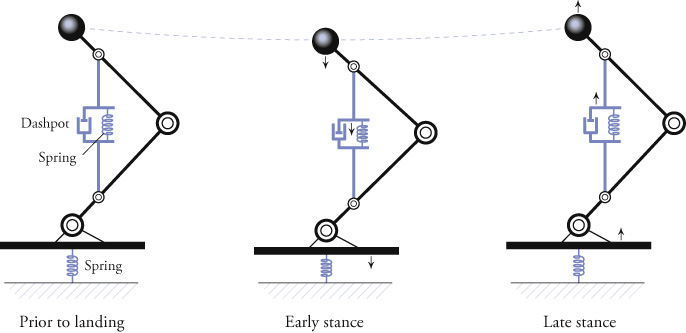
\includegraphics[width=1.0\linewidth]{chap3/3_10}
	\caption{McMahon 和 Greene 用于预测在柔顺跑道上跑步表现的概念模型。
		被动弹簧减震器系统代表肌肉的机械特性,脚下的弹簧代表跑道的柔顺性。
		分析了该系统在站立初期(中)的压缩和站立后期(右)的回弹动态,以找到最适合腿部特性的跑道弹簧刚度\cite{mcmahon1979influence}。 \label{fig:3_10}}
\end{figure}

该系统具有 2 个自由度,其动力学由两个二阶常微分方程控制,可从图~\ref{fig:3_11}~所示的示意图推导出来:

\begin{figure}[!htb]
	\centering
	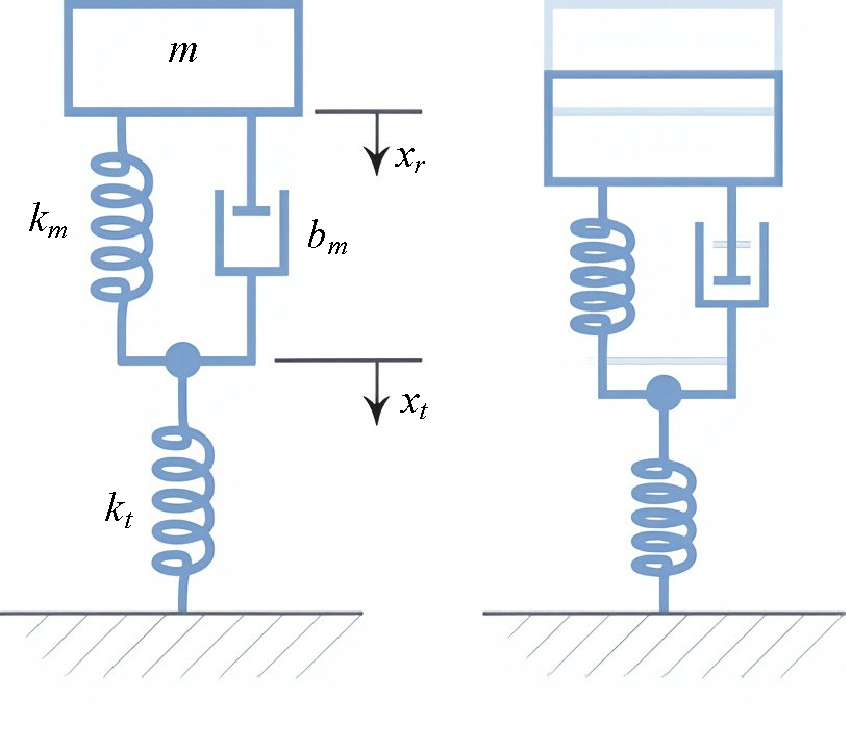
\includegraphics[width=0.4\linewidth]{chap3/3_11}
	\caption{用于推导图~\ref{fig:3_10}~所示概念模型运动方程的示意图。
		左图为系统处于平衡状态,右图为系统处于站立状态。
		跑步者的身体被建模为一个质量块 ($m$),其在弹簧(刚度为 $k_m$)和阻尼器(阻尼系数为 $b_m$)产生的力(代表腿部肌肉的综合作用)的作用下,发生位移 $x_r$ 的移动。
		脚下的小块跑道被建模为一个无质量物体,并通过一个代表跑道柔度的弹簧(刚度为 $k_t$)连接到地面\cite{mcmahon1979influence}。 \label{fig:3_11}}
\end{figure}

\begin{equation}
\begin{aligned}
	m \ddot{x}_t + 
	m_m ( \dot{x}_r - \dot{x}_t )
	k_m ( x_r - x_t ) = 0 \\
	b_m ( \dot{x}_r - \dot{x}_t )
	+ k_m ( x_r - x_t ) 
	- k_t x_t = 0
\end{aligned}
\end{equation}
% 
其中 $m$ 是跑步者身体的质量,$x_r$ 是其相对于平衡位置的位移,$x_t$ 是脚下跑道的位移,$b_m$ 是减震器的阻力,$k_m$ 和 $k_t$ 分别是肌肉和跑道弹簧的刚度。


McMahon 和 Greene 通过计算该系统的固有频率,并注意到足部在大约一次振动周期的一半后便会抬离地面,从而估算出了足部与地面的接触时间,该接触时间与履带刚度 $k_t$ 的关系。
他们的第一个意外发现是,在一系列中等刚度的履带上,接触时间比在非常坚硬的路面(例如混凝土路面)上跑步时的接触时间更短($t_0$;图~\ref{fig:3_12})。
即使步幅保持不变,这一发现也令人预期跑步速度会有所提升,因为步频往往会随着接触时间的减少而增加。

\begin{figure}[!htb]
	\centering
	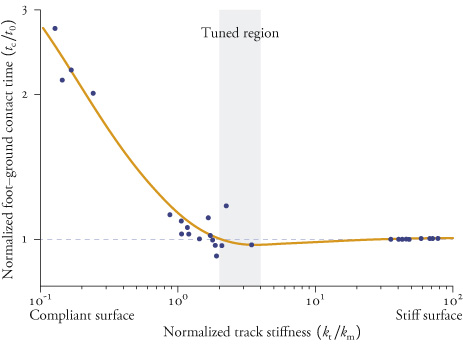
\includegraphics[width=1.0\linewidth]{chap3/3_12}
	\caption{足部触地时间与履带刚度的关系。
		两个坐标轴均为对数刻度。
		足部触地时间 ($t_c$) 由硬地面上的触地时间 ($t_0$) 归一化;履带刚度 ($k_t$) 由腿部刚度 ($k_m$) 归一化。
		实线由图~\ref{fig:3_11}~所示的模型确定,使用阻尼比为 ${b_m} / {2\sqrt{m k_m}} = 0.55$,因为该值与实验数据拟合度最高。
		调整区域(阴影部分)显示了减少触地时间的潜力\cite{mcmahon1984muscles}。 \label{fig:3_12}}
\end{figure}

但还有更好的消息。
他们的模型过于简单,无法预测步幅,因此 McMahon 和 Greene 构建了各种刚度的跑步表面,从几乎刚性到非常柔顺的蹦床跑道,并估算了人们在这些表面上跑步时的步幅。
正如预期的那样,与在刚性表面上跑步相比,在非常柔顺的表面上跑步的步幅显著增加(图~\ref{fig:3_13})。
但当然,在蹦床上跑步太慢了,因为脚和蹦床之间的接触时间大大增加。
最相关的发现是,即使在“调整区域”(在图~\ref{fig:3_12}~和图~\ref{fig:3_13}~中以灰色条纹显示),接触时间也减少了,步幅仍然增加了约 1\%。
这是一个双赢的区域,步幅和步频都得到了增强。对于刚度在这个区域内的跑道,大约是跑步者腿部刚度的 2 到 4 倍,我们预计跑步速度会增加(相比之下,混凝土的硬度是人腿的 100 倍)。

\begin{figure}[!htb]
	\centering
	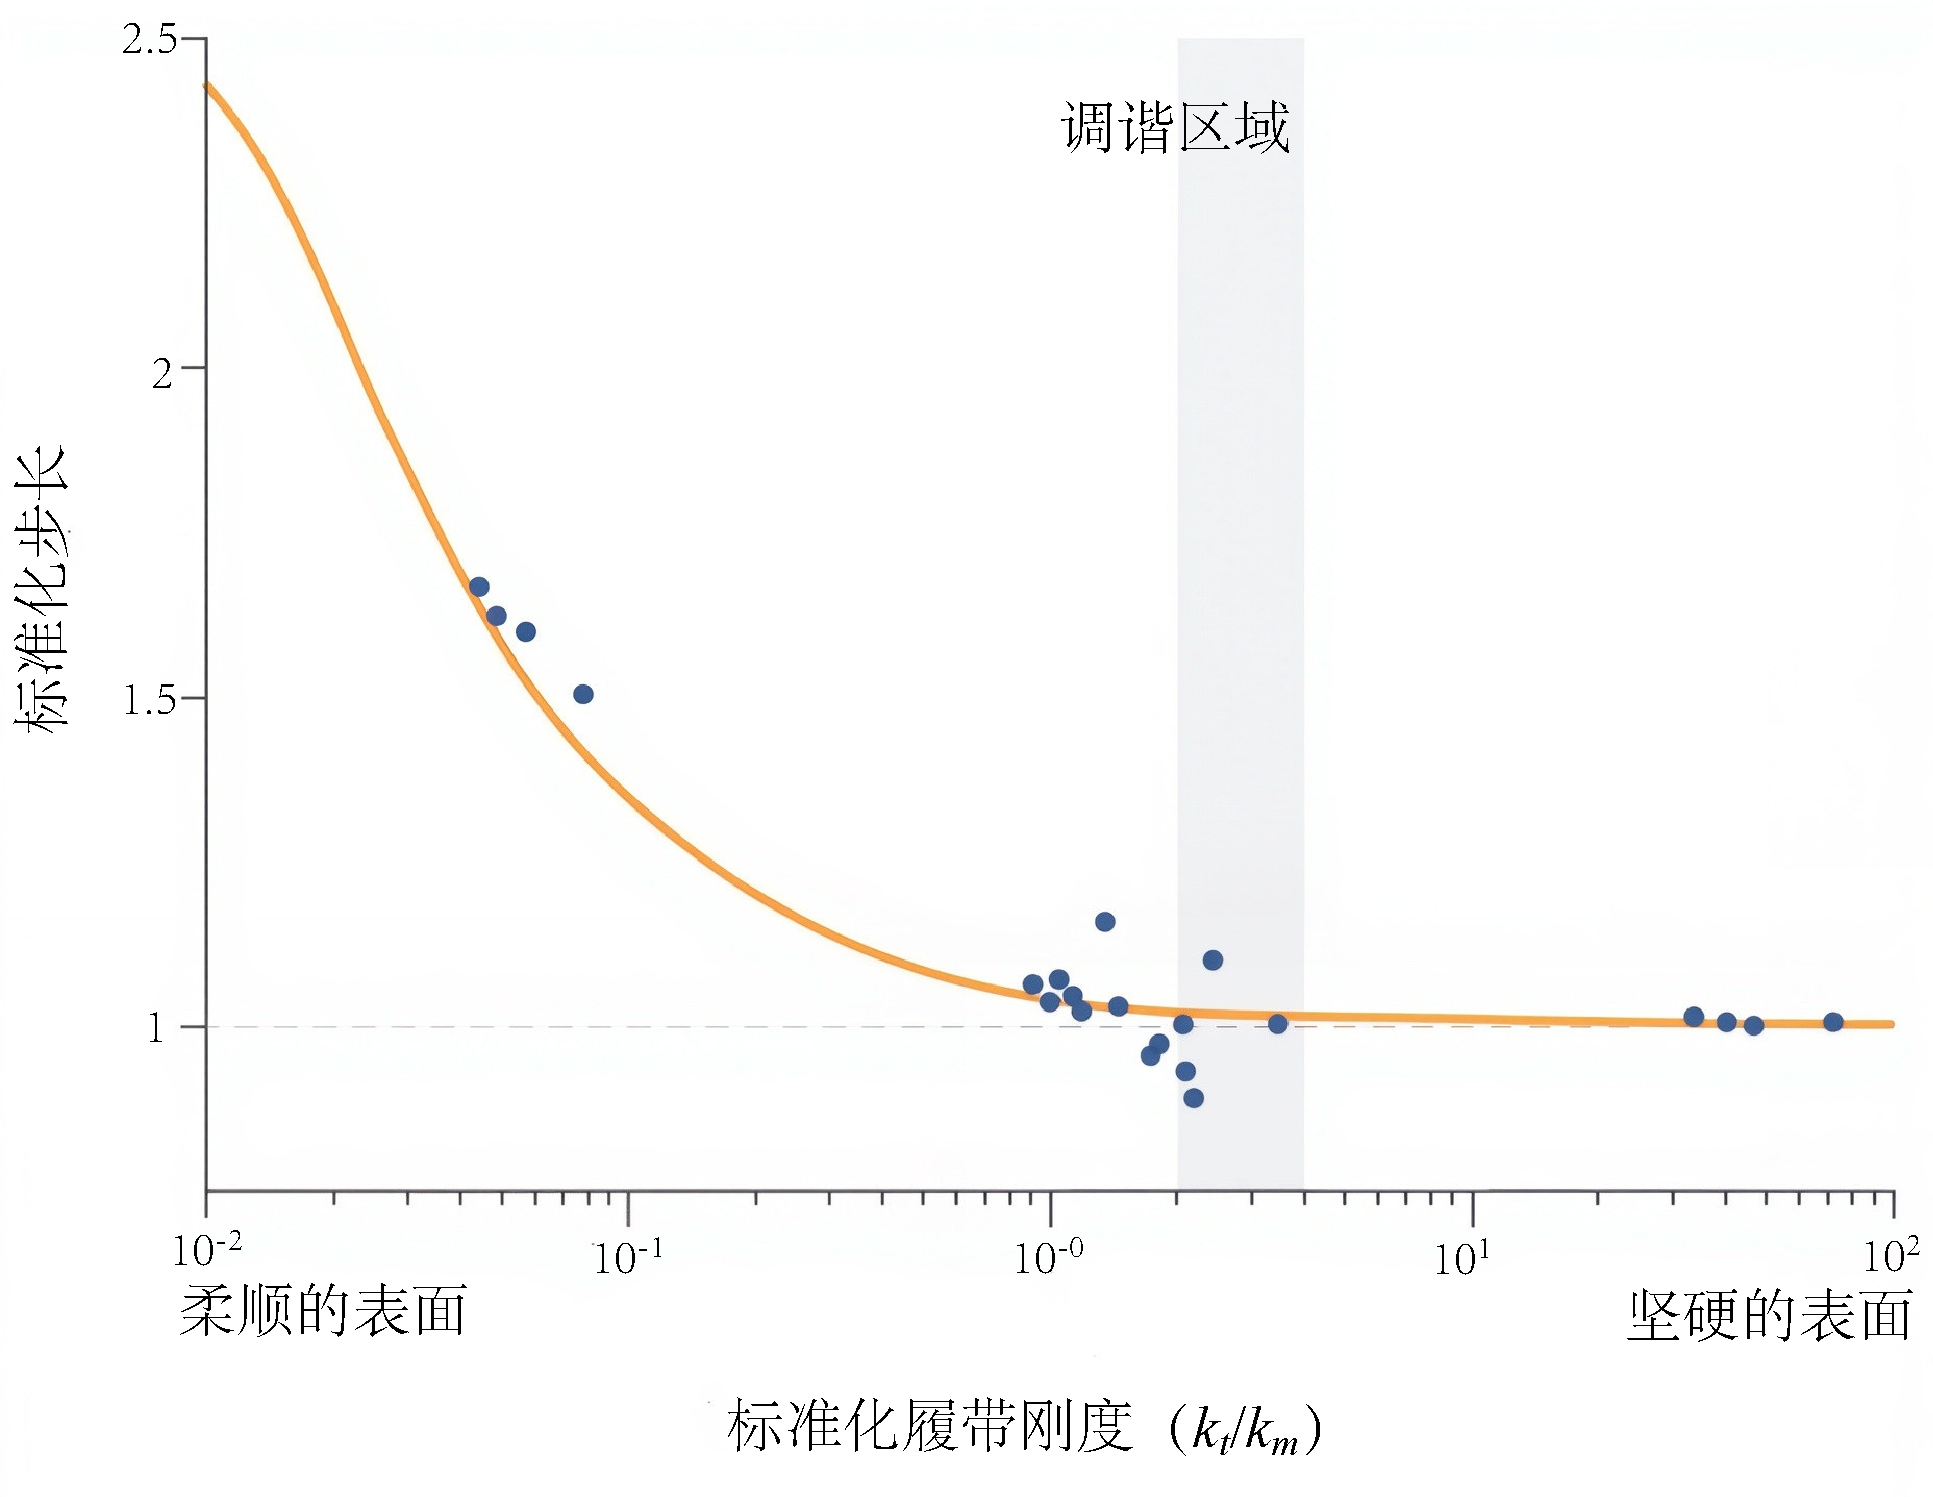
\includegraphics[width=1.0\linewidth]{chap3/3_13}
	\caption{步长(以硬路面上的步长为标准)与履带刚度(以腿部刚度为标准)的关系。
		图中点表示与曲线最接近的实验步长。
		调整区域(阴影部分)与图~\ref{fig:3_12}~所示相同。
		在此区域,步长约增加了 1\% \cite{mcmahon1984muscles}。 \label{fig:3_13}}
\end{figure}

哈佛大学、耶鲁大学、麦迪逊广场花园和新泽西州的梅多兰兹体育馆都建造了刚度达到该范围内的室内跑道。
哈佛大学的跑道设计刚度约为190千牛/米,对于体重75公斤的跑步者来说,跑道挠度约为8毫米(假设跑步者在站立中段承受两倍于其体重的力,如图3.3所示)。
跑步者不仅将时间提高了约2\%或3\%(约每英里5秒),而且受伤率也降低了,这可能是因为在经过调整的跑道上落地更轻柔。


如今的跑道建造非常注重跑道回馈给跑步者的能量。
毫无疑问,它们的建造比1977年启用的哈佛跑道更为复杂。
即使麦克马洪的研究成果已不再代表当时的先进水平,他对跑步的分析以及对调校跑道的设计,仍然是用简单模型就能获得高里程的绝佳范例。
类似的分析也可用于设计跑鞋,我们接下来会看到。


\section{改进跑鞋的弹性机制}

Rodger Kram 和他的同事评估了耐克的一款原型跑鞋,这款跑鞋的弹性泡沫中底嵌入了一块碳纤维板,用于储存和释放弹性能量。
当对鞋子施加力时,鞋子会变形;分析力与变形的关系可以告诉我们一些有关弹性能量的储存和释放的信息。
将原型鞋与马拉松运动员使用的标准跑鞋进行比较表明,原型鞋在变形时储存了更多的弹性能量,而在回弹时释放了更高比例的能量(图~\ref{fig:3_14})。
当 18 名精英运动员穿着这双鞋跑步时,与标准马拉松跑鞋相比,他们的跑步能量成本平均降低了 4\%,这与四十年前调谐跑道带来的优势相似。

\begin{figure}[!htb]
	\centering
	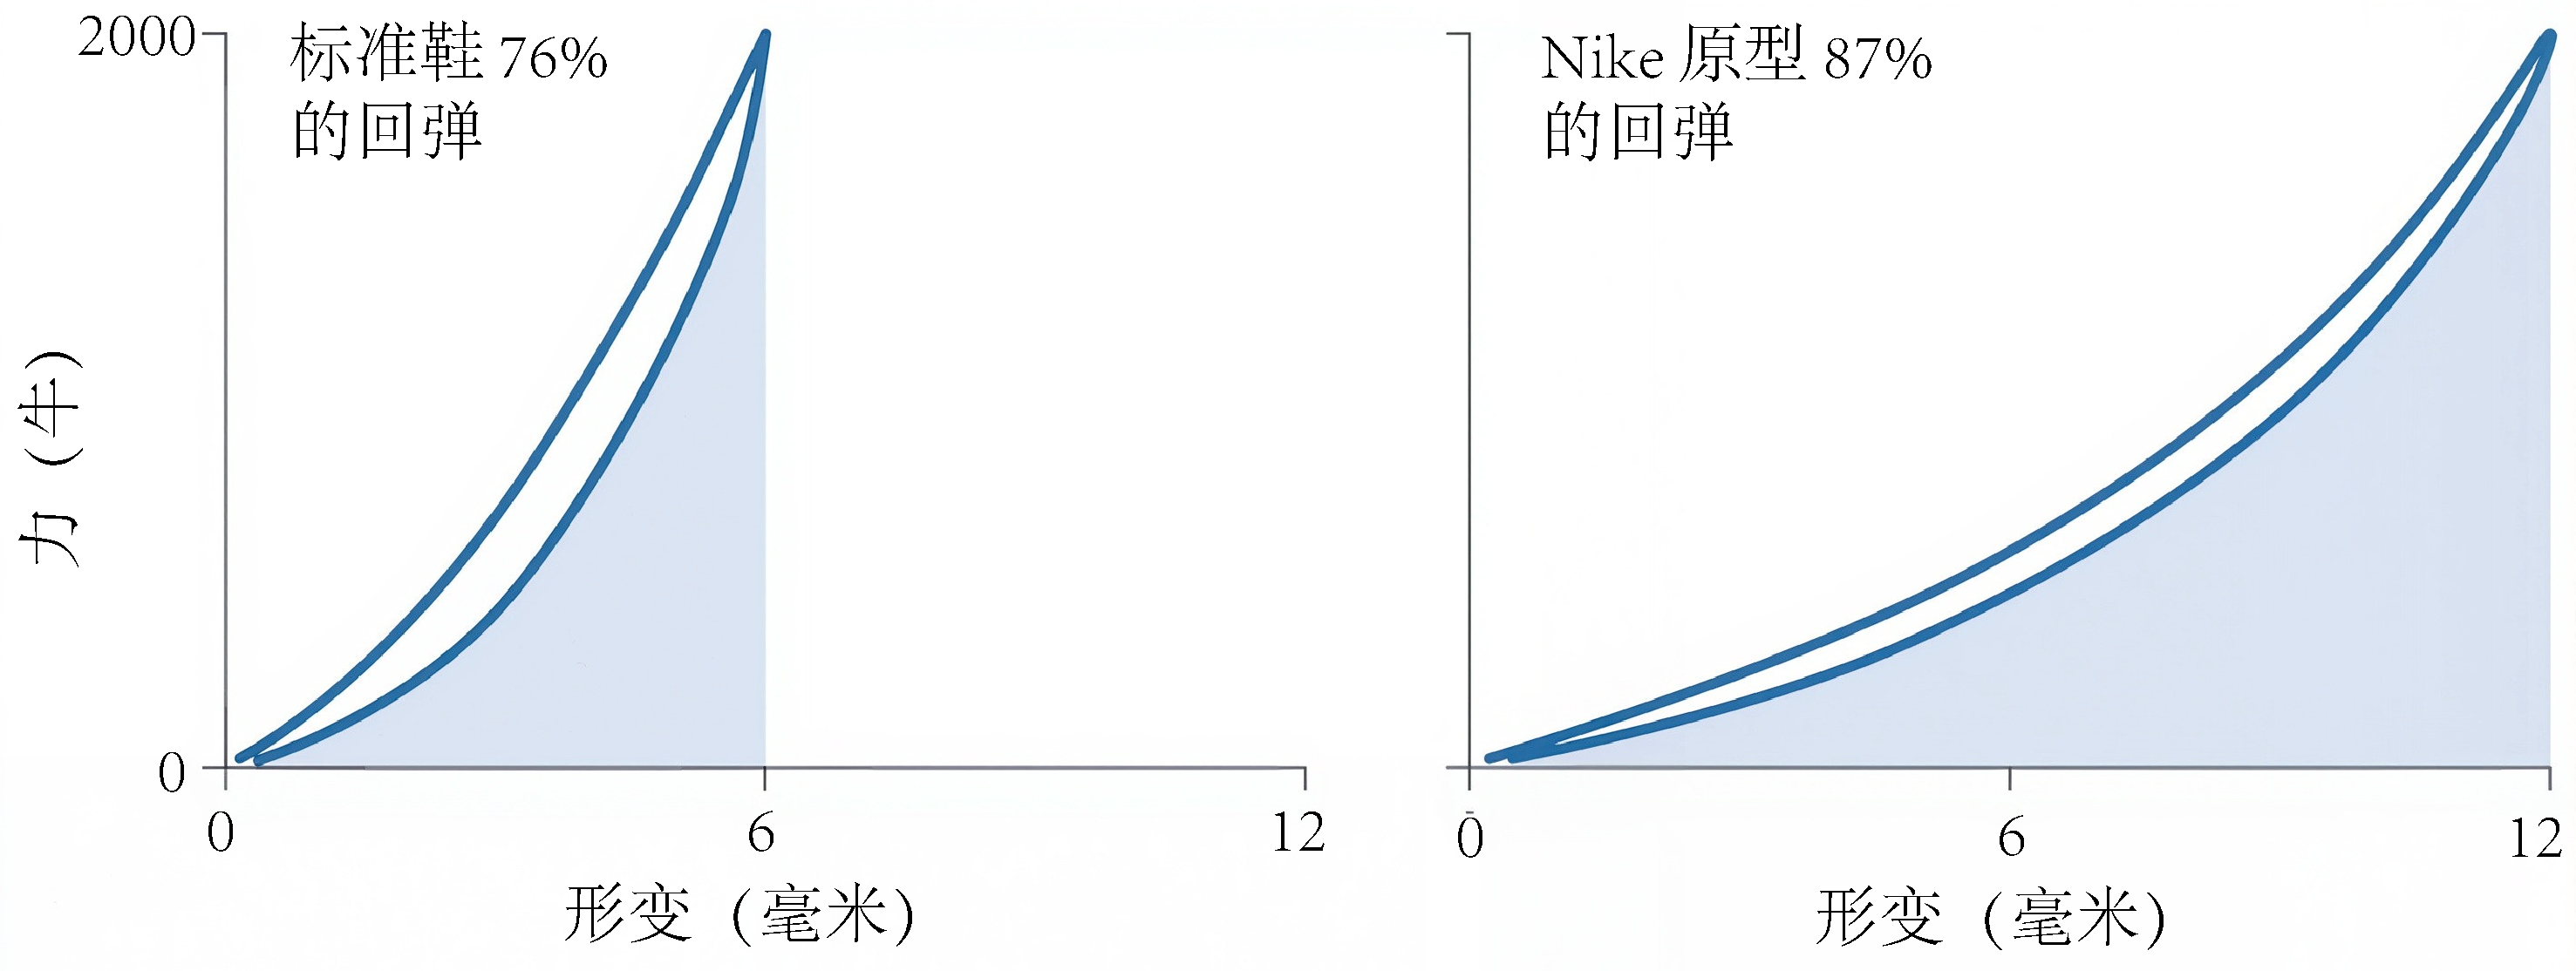
\includegraphics[width=1.0\linewidth]{chap3/3_14}
	\caption{两双跑鞋的力-变形曲线。当力作用于每只跑鞋时,鞋子都会变形(每条曲线的上方轨迹)。
		然后,当鞋子卸载时,中底会回弹(每条曲线的下方轨迹)。
		加载和卸载曲线之间的区域表示以热量形式损失的机械能。
		下方轨迹下方的区域(阴影部分)表示鞋子卸载时返回的弹性能量\cite{hoogkamer2018comparison}。 \label{fig:3_14}}
\end{figure}


\section{腿部僵硬程度随体重变化}

质量-弹簧模型分析表明,许多动物的腿部僵硬程度都与体重成正比\cite{farley1993running}。
例如,松鼠体重较小,行走时四肢弯曲柔顺,而大象体重较大,则更喜欢用更直的腿行走。
负重跑步会人为地增加体重,这在人类中很常见,因此,探索体重如何影响人类跑步过程中腿部僵硬程度是一个有趣的场景。
艾米$\cdot$西尔德 (Amy Silder) 在我位于斯坦福大学的实验室工作时,收集了业余跑步者的数据。
每位受试者都以自己舒适的训练速度 (3.34 ± 0.22 米/秒) 在装有测力板的跑步机上跑步。
受试者分别在不负重以及穿着背心时负重 10\%、20\% 或 30\% 的体重跑步。
无量纲腿部刚度($k_\text{leg}$)估计为:以体重($F_\text{peak}$)标准化的峰值垂直地面反作用力与站立阶段腿部长度变化(以脚接触时的腿部长度标准化)($l_0$)之比:
%
\begin{equation}
	k_\text{leg} = \frac{F_\text{peak}}{l_\text{min} / l_0 }
\end{equation}
%
其中$l_\text{min}$是站立时腿的最小长度。
腿长定义如图~\ref{fig:3_15}~所示。

\begin{figure}[!htb]
	\centering
	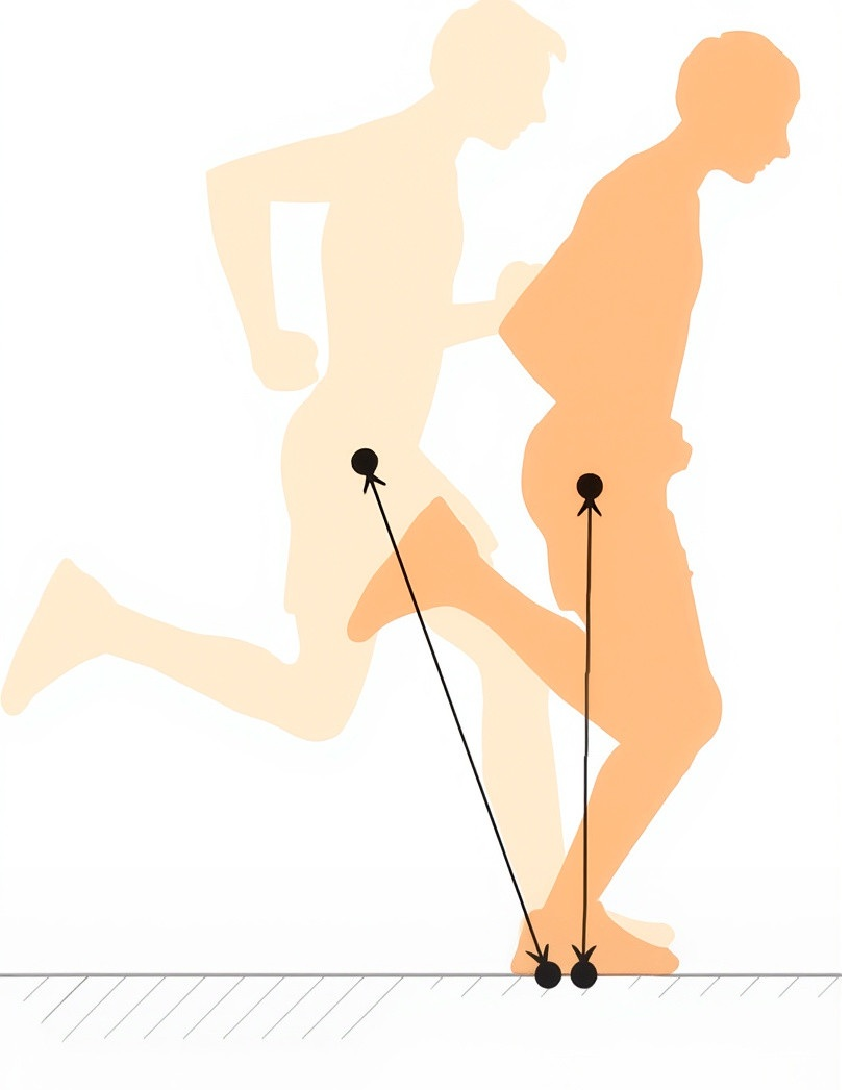
\includegraphics[width=0.4\linewidth]{chap3/3_15}
	\caption{腿长定义为压力中心和骨盆几何中心之间的距离。 \label{fig:3_15}}
\end{figure}

这些实验表明,负重跑步时,无量纲腿部刚度会增加,因为峰值垂直地面反作用力会增加,而支撑相腿长的变化会减小(图~\ref{fig:3_16})。
这些实验与 Farley 等人\cite{farley1993running} 指出的趋势相符,即腿部刚度会随着体重的增加而增加。

\begin{figure}[!htb]
	\centering
	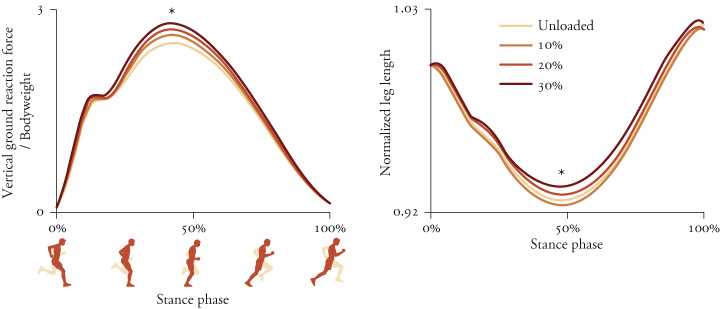
\includegraphics[width=0.4\linewidth]{chap3/3_16}
	\caption{站立期,以体重(左)归一化的垂直地面反作用力,以及以足触地时腿长(右)归一化的腿长。
		受试者分别在无负重和穿着负重分别为其体重 10\%、20\% 或 30\% 的背心跑步。
		随着负重增加,峰值垂直地面力增加(p < 0.001),腿长变化减小(p = 0.025)\cite{silder2015running}。 \label{fig:3_16}}
\end{figure}

腿部僵硬程度也可能因所穿跑鞋的类型而变化。
跑鞋的缓冲功能通常用于减少冲击负荷,正如我们在上文描述的调整跑道中看到的那样。
然而,Kulmala 及其同事\cite{kulmala2018running}报告称,与传统跑鞋相比,穿着高缓冲跑鞋跑步会增加腿部僵硬程度,并增大冲击负荷。
因此,在尝试减少跑步过程中的肌肉骨骼负荷时,需要考虑跑鞋力学与肢体僵硬程度之间复杂的相互作用。


\section{步态转换}

随着步行速度的增加,支撑期缩短;
最终,双支撑期完全消失,形成腾空期(图~\ref{fig:3_17})。
研究从步行到跑步的过渡过程中地面反作用力的变化情况很有意思。
在低速步行时,支撑期较长,双支撑期也较长。
随着步行速度的增加,地面反作用力在整个步态周期中的变化增大,双支撑期缩短。
以超过 2 米/秒的速度行走很困难;
即使没有腾空期,峰值地面反作用力也会远高于体重,并且在整个步态周期中变化很大。
在更高的速度下,你甚至无法行走,只能开始跑步。
由于足部与地面接触的时间如此之短,峰值地面反作用力会急剧增加,超过体重的 2 倍。
一个重要的问题是:是什么驱动了这种步态之间的转变?
比较不同动物的步态可以提供重要的线索。


\begin{figure}[!htb]
	\centering
	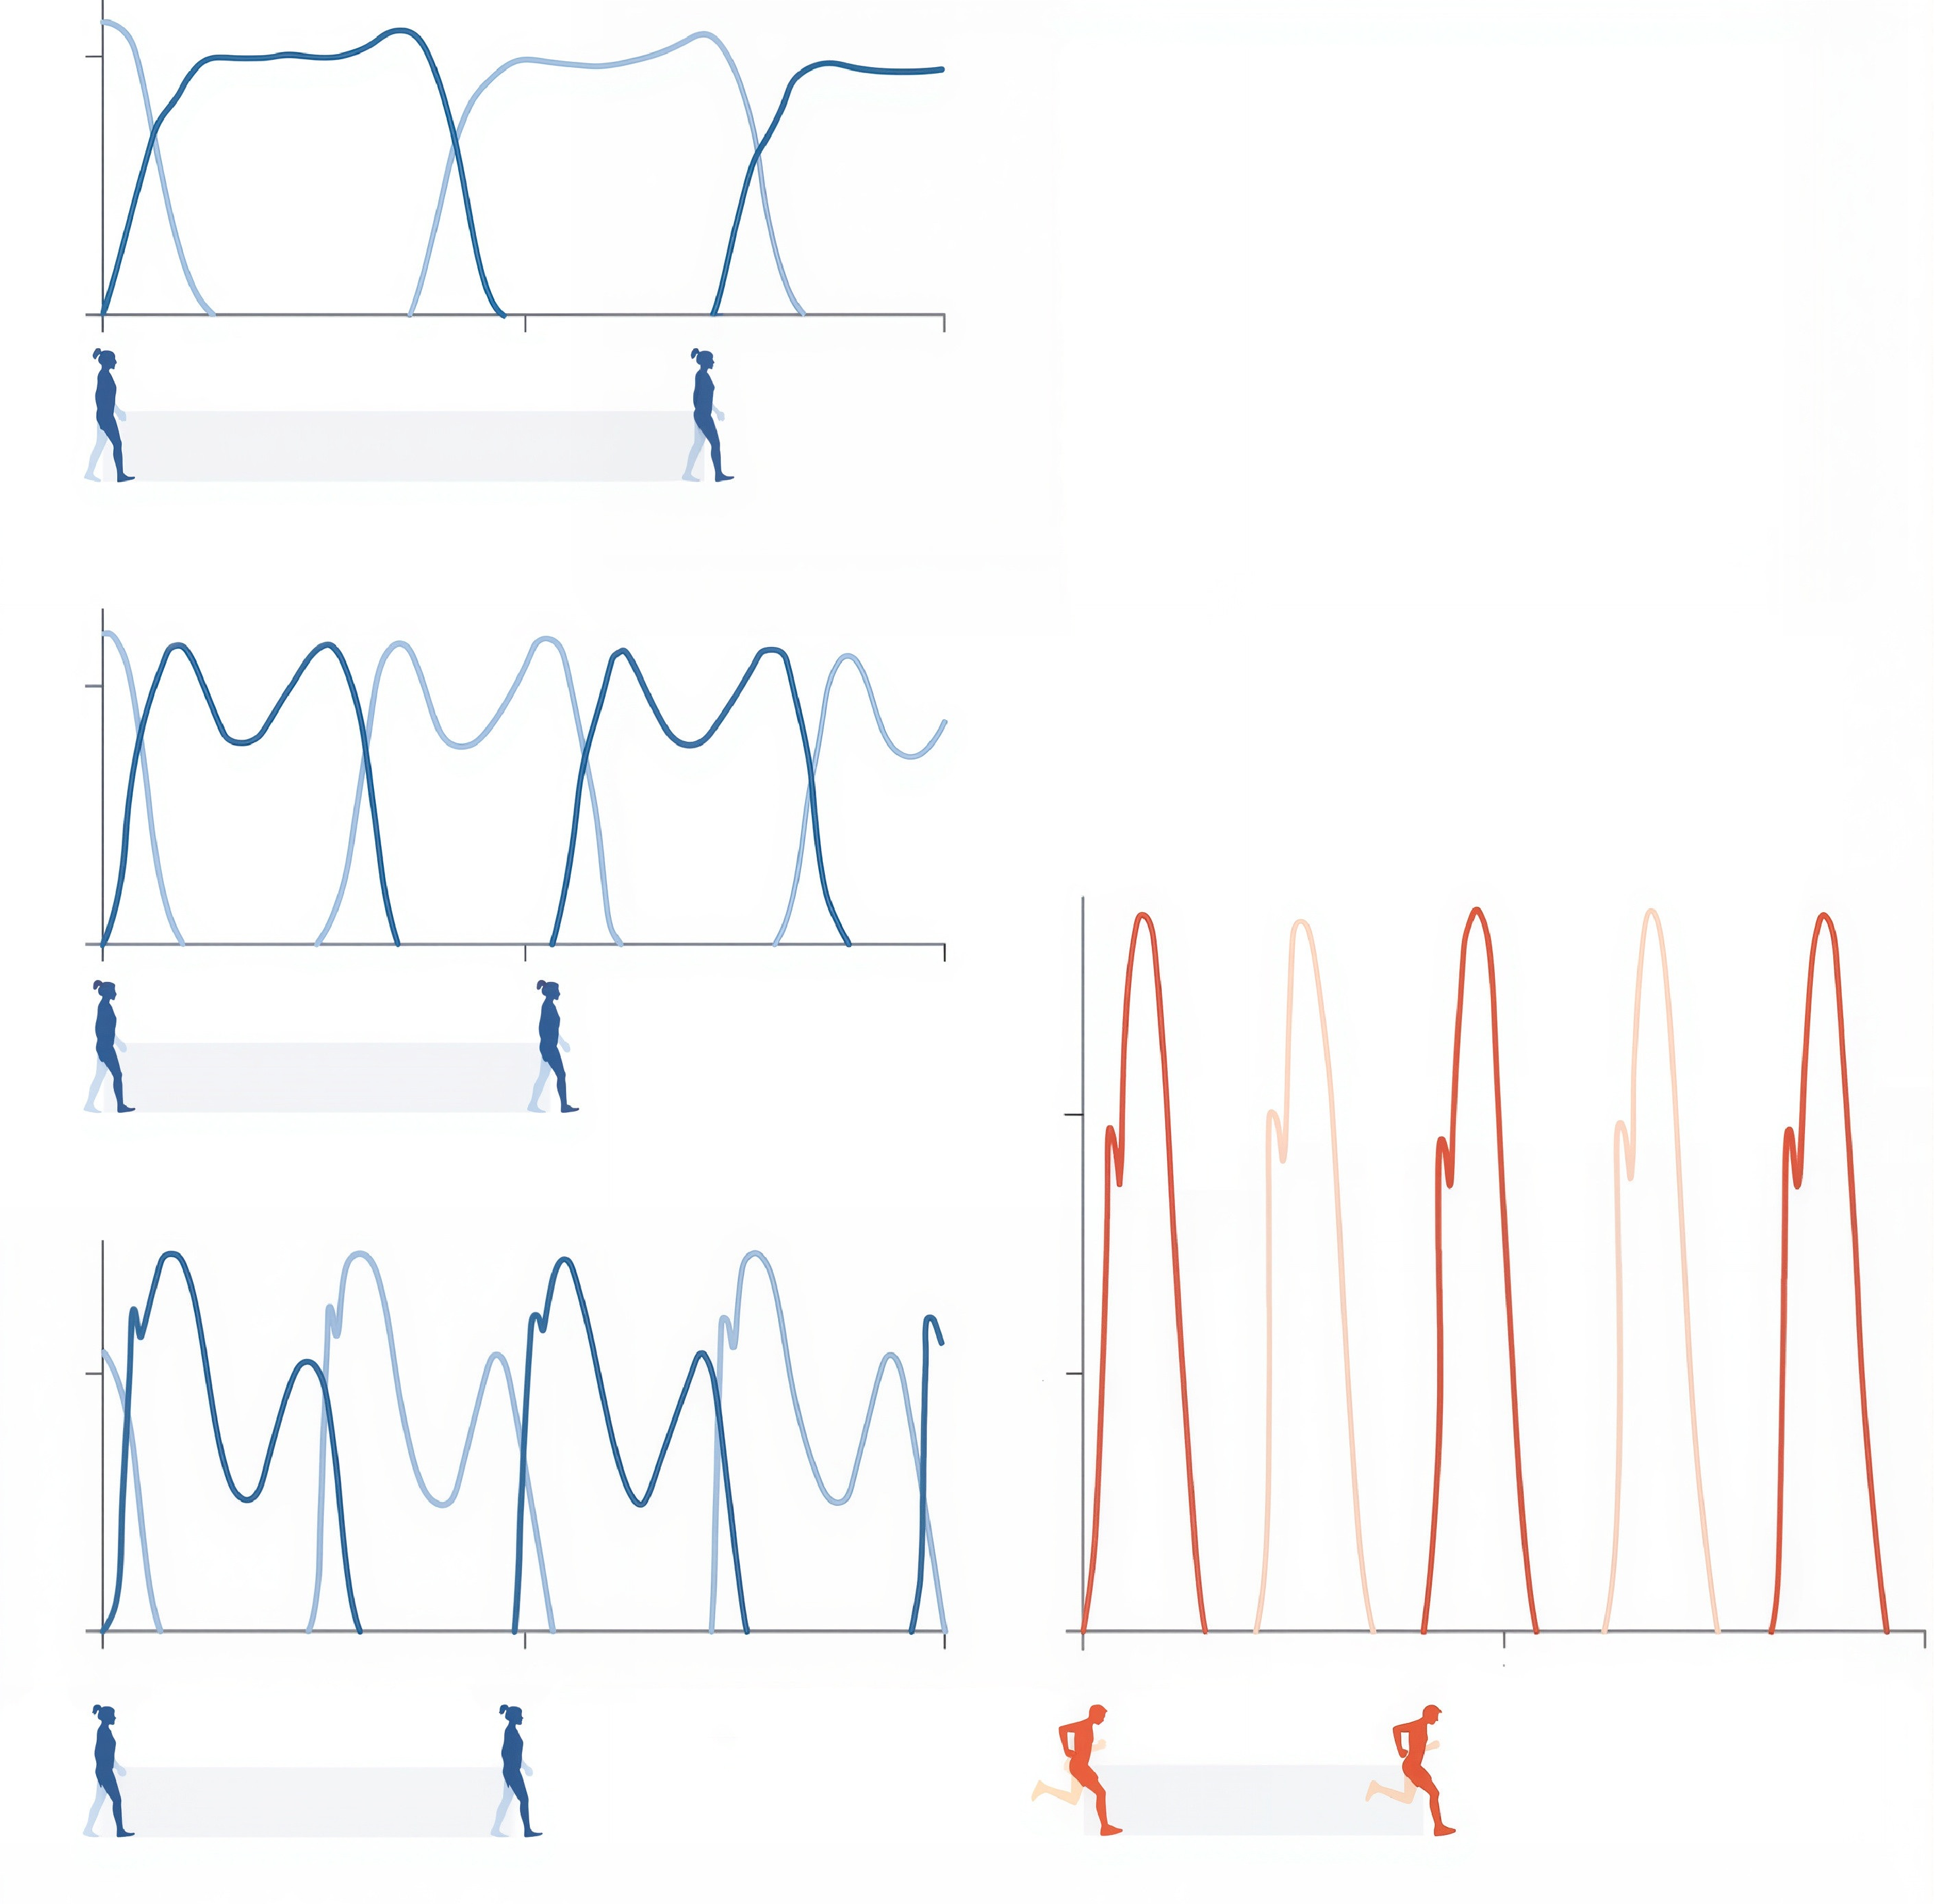
\includegraphics[width=1.0\linewidth]{chap3/3_17}
	\caption{地面反作用力的垂直分量随速度增加而变化。
		左图从上到下:慢速、中速和快速行走;
		右图:跑步\cite{alexander1984walking}。 \label{fig:3_17}}
\end{figure}


当以特定速度移动时,人类和其他动物通常会选择运输成本最低的运动方式。
例如,随着速度的增加,马会从步行过渡到小跑,再到飞奔(图~\ref{fig:3_18})。
虽然它们会根据期望的速度调整步态,但反之亦然:
一旦选择了特定的步态,它们就会倾向于以该步态下运输成本最低的速度行进。
例如,马的行走速度通常约为 1.25 米/秒,这是图~\ref{fig:3_18}~中蓝色曲线的最低点。
类似地,人类也会从步行过渡到跑步,此时跑步的速度更经济。
请注意,如果您需要在固定的时间内覆盖特定的距离,那么舒适地步行一段路程,然后跑步完成剩余路程可能比全程快速行走或慢跑更节省能量。
与步行一样,我们自然会选择步长和步频等变量来最小化以特定速度跑步时的能量消耗。

\begin{figure}[!htb]
	\centering
	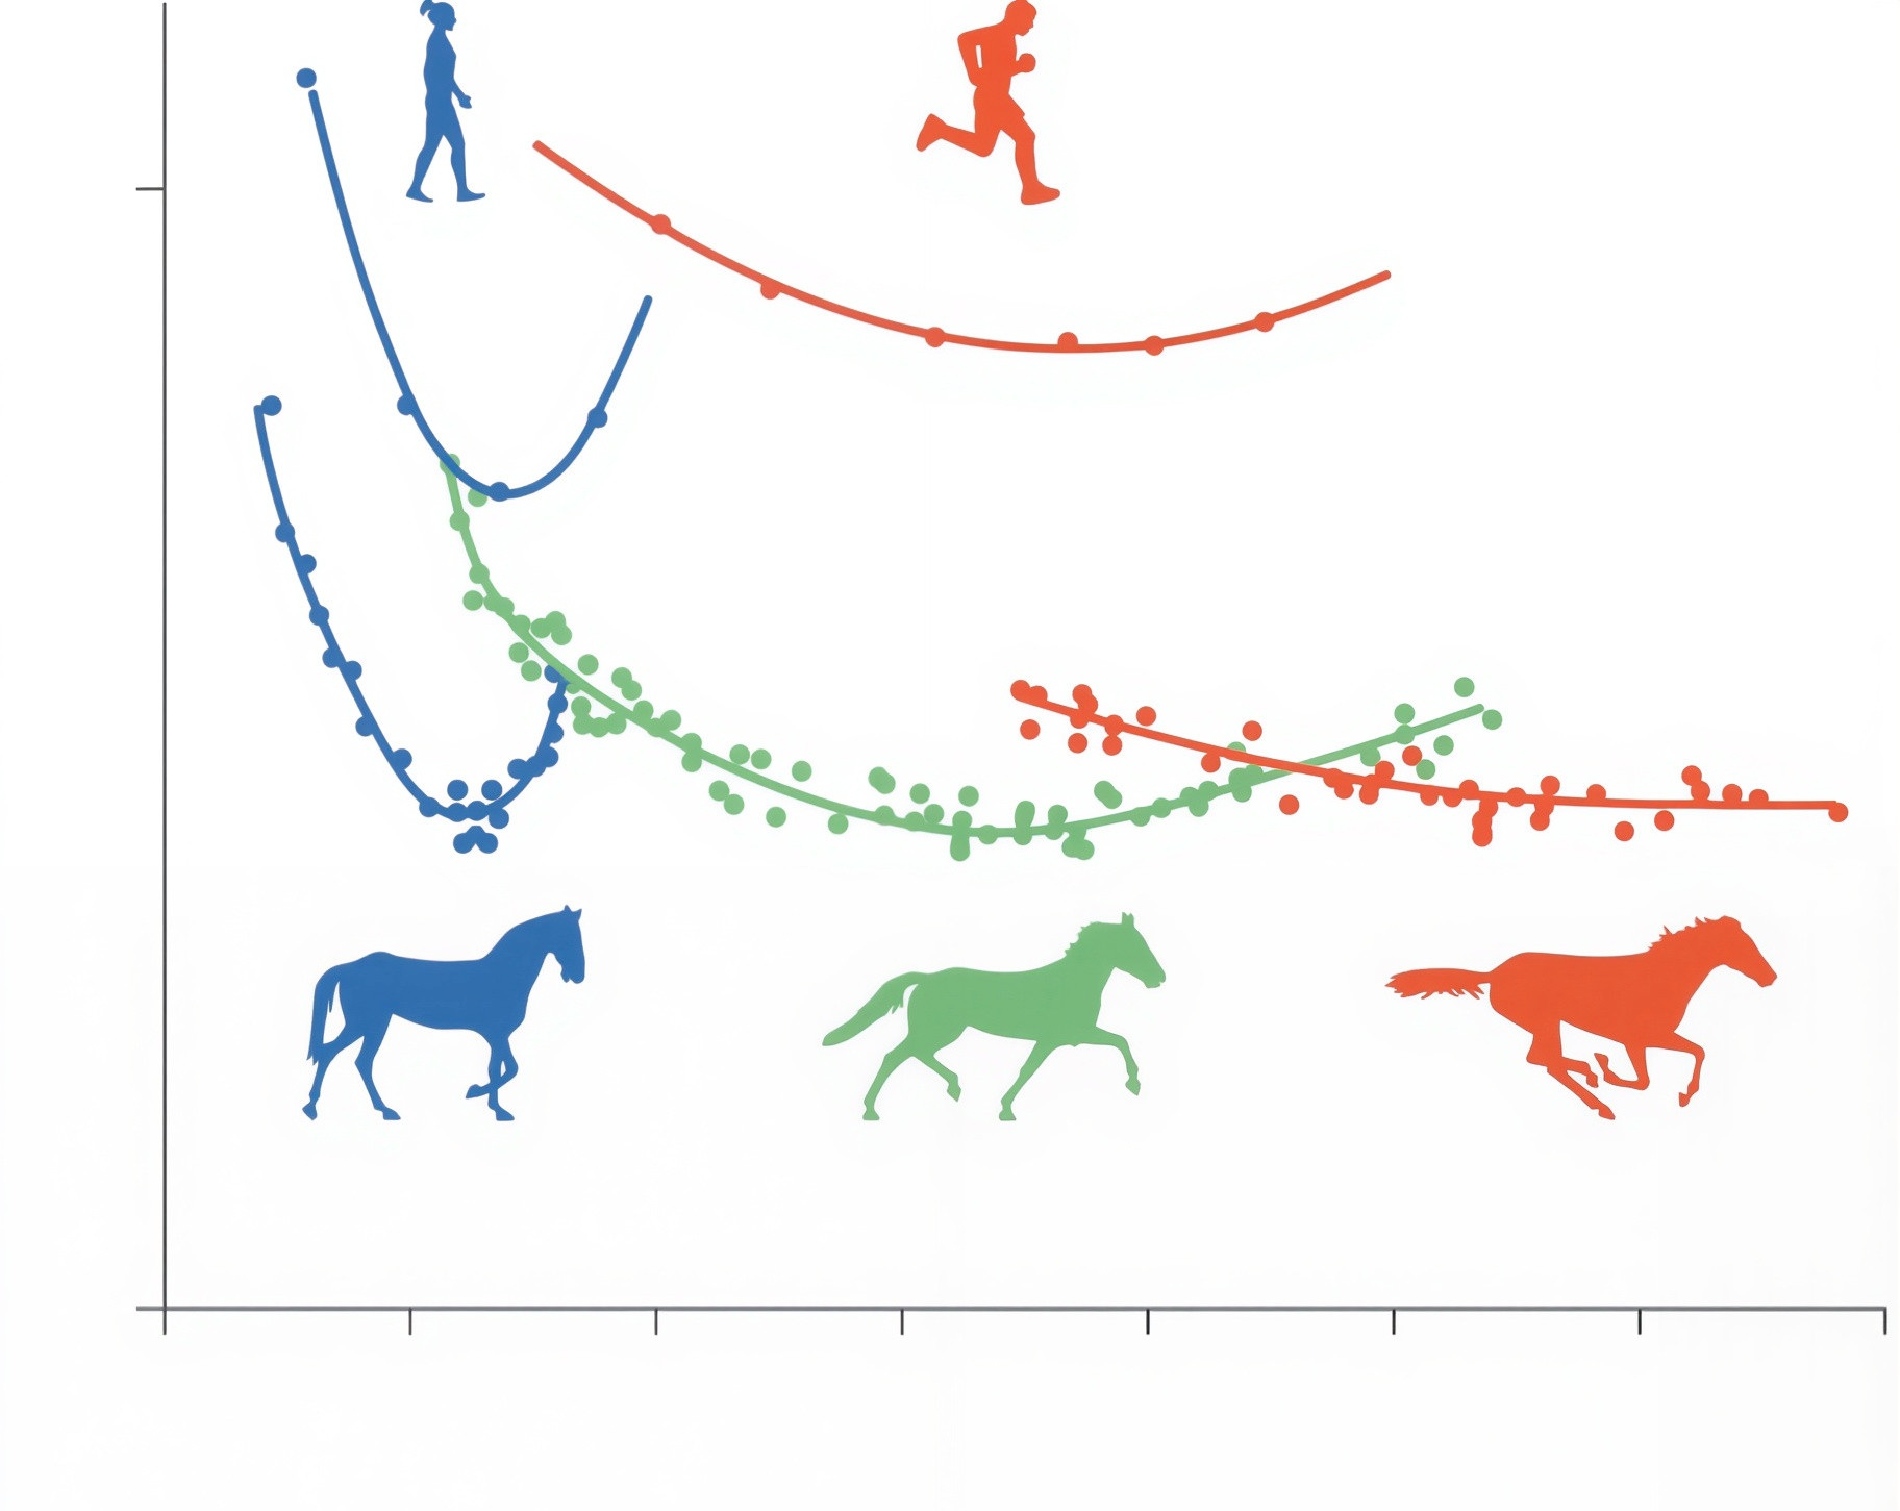
\includegraphics[width=0.85\linewidth]{chap3/3_18}
	\caption{地面反作用力的垂直分量随速度增加而变化。
		左图从上到下:慢速、中速和快速行走;
		右图:跑步\cite{alexander1984walking}。 \label{fig:3_18}}
\end{figure}


\section{双足质量弹簧模型}

在第~\ref{chap:chap2}~章中,我们将行走建模为具有刚性腿的倒立摆运动;
在本章中,我们将跑步建模为具有柔顺腿的弹跳步态。
每种模型都有其优势,但也存在一些重要的局限性。
2006年,Hartmut Geyer、Andre Seyfarth 和 Reinhard Blickhan 提出了一个统一的行走和跑步模型,通过引入两条柔顺腿克服了部分局限性(图~\ref{fig:3_19})。
该模型再现了跑步的 3 个重要特征:地面反作用力、弹性能量储存以及站立和腾空交替的跑步步态周期。
有趣的是,该模型还展示了行走特有的前向动能和重力势能的异相波动。
对该模型的分析表明,行走效率取决于沿着倒立摆弧线的质心轨迹以及腿部弹簧中的弹性能量储存。
双支撑过程中原本会损失的能量可以通过腿部弹簧中储存的能量进行回收。
拥有一个可以同时产生步行和跑步的单一模型表明这些步态比以前认为的更相似。

\begin{figure}[!htb]
	\centering
	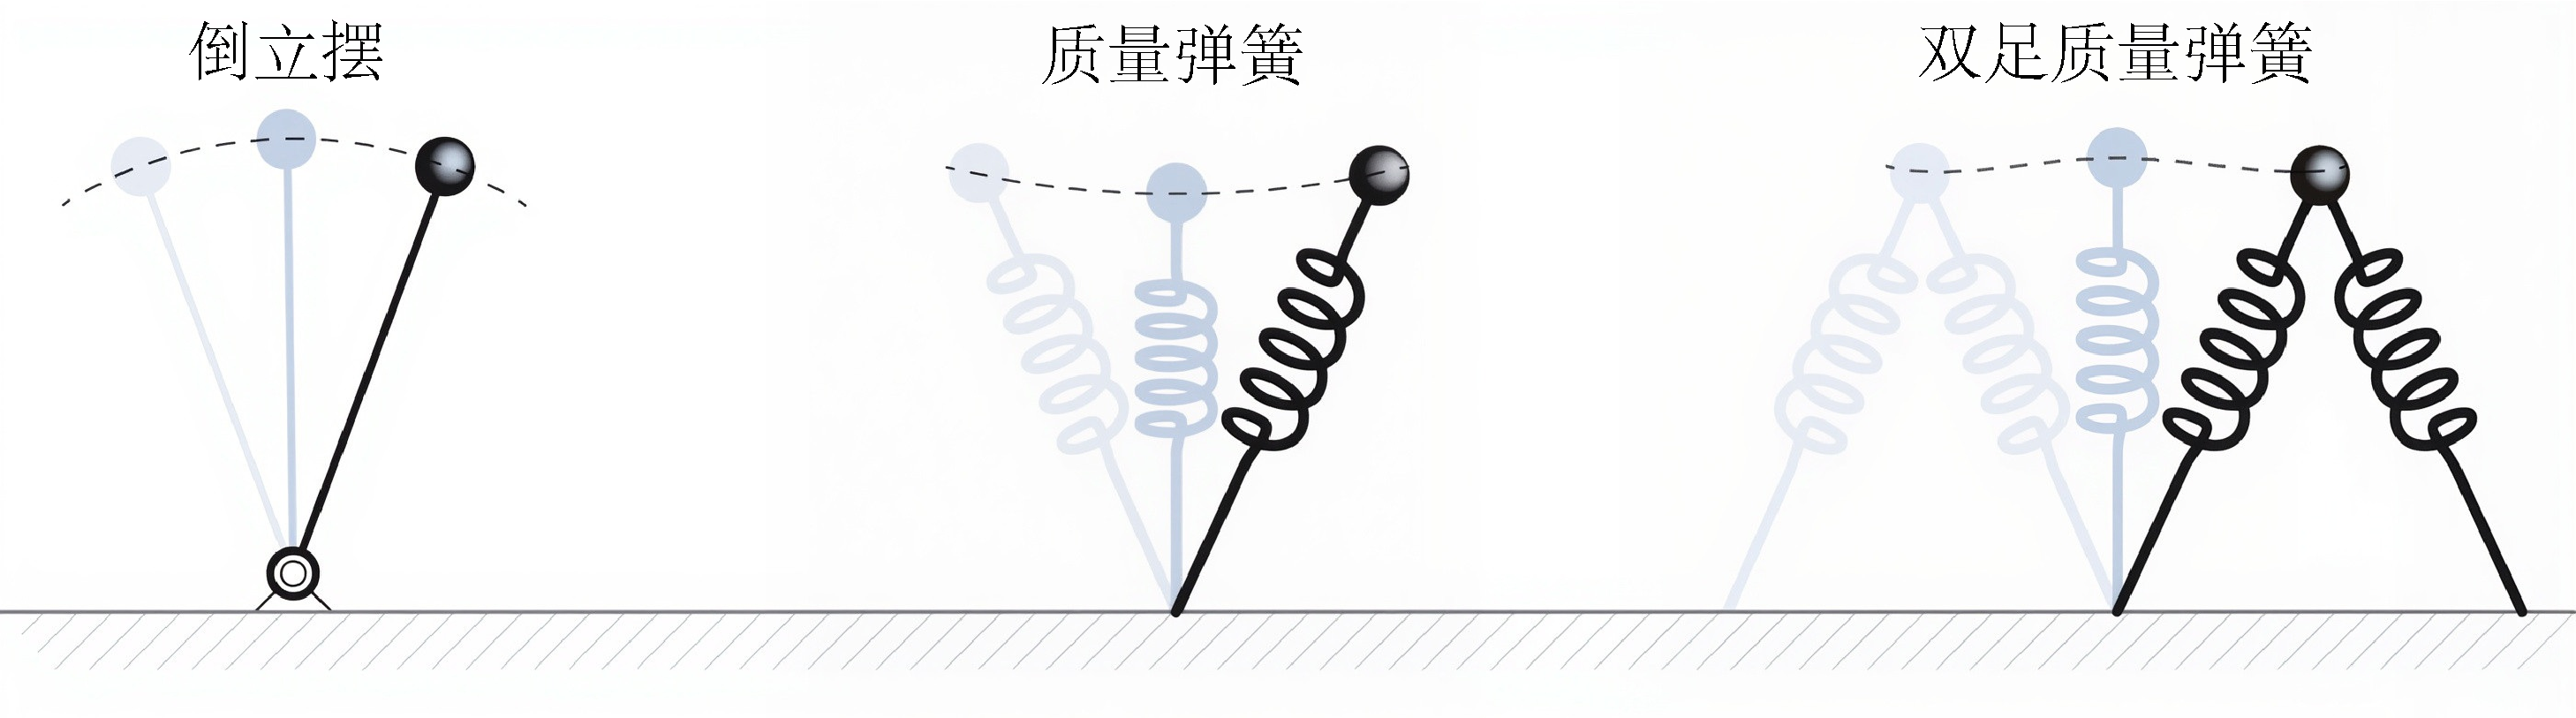
\includegraphics[width=1.0\linewidth]{chap3/3_19}
	\caption{用僵硬腿行走的倒立摆模型(左)和用柔顺腿跑步的质量弹簧模型(中)可以组合成一个双足质量弹簧模型,用于解释行走和跑步的基本动力学(右)。
		右图显示了行走过程中的质心轨迹\cite{geyer2006compliant}。 \label{fig:3_19}}
\end{figure}


\section{跑步运动学}

除了理解跑步过程中地面反作用力和能量消耗之外,理解跑步运动学也至关重要。
也就是说,我们想要了解图~\ref{fig:2_17}~中所示的关节如何运动:它们何时弯曲、何时伸展以及伸展的幅度。
使用我们将在第~\ref{chap:chap7}~章中介绍的运动捕捉方法,我们可以估算跑步过程中发生的关节角度,并描述关节运动如何随跑步速度而变化。
图~\ref{fig:3_20}~显示了采用后脚掌着地跑步姿势的受试者的典型结果。
跑步时关节运动范围比行走时更大,并且运动范围会随着跑步速度的增加而增大。


\begin{figure}[!htb]
	\centering
	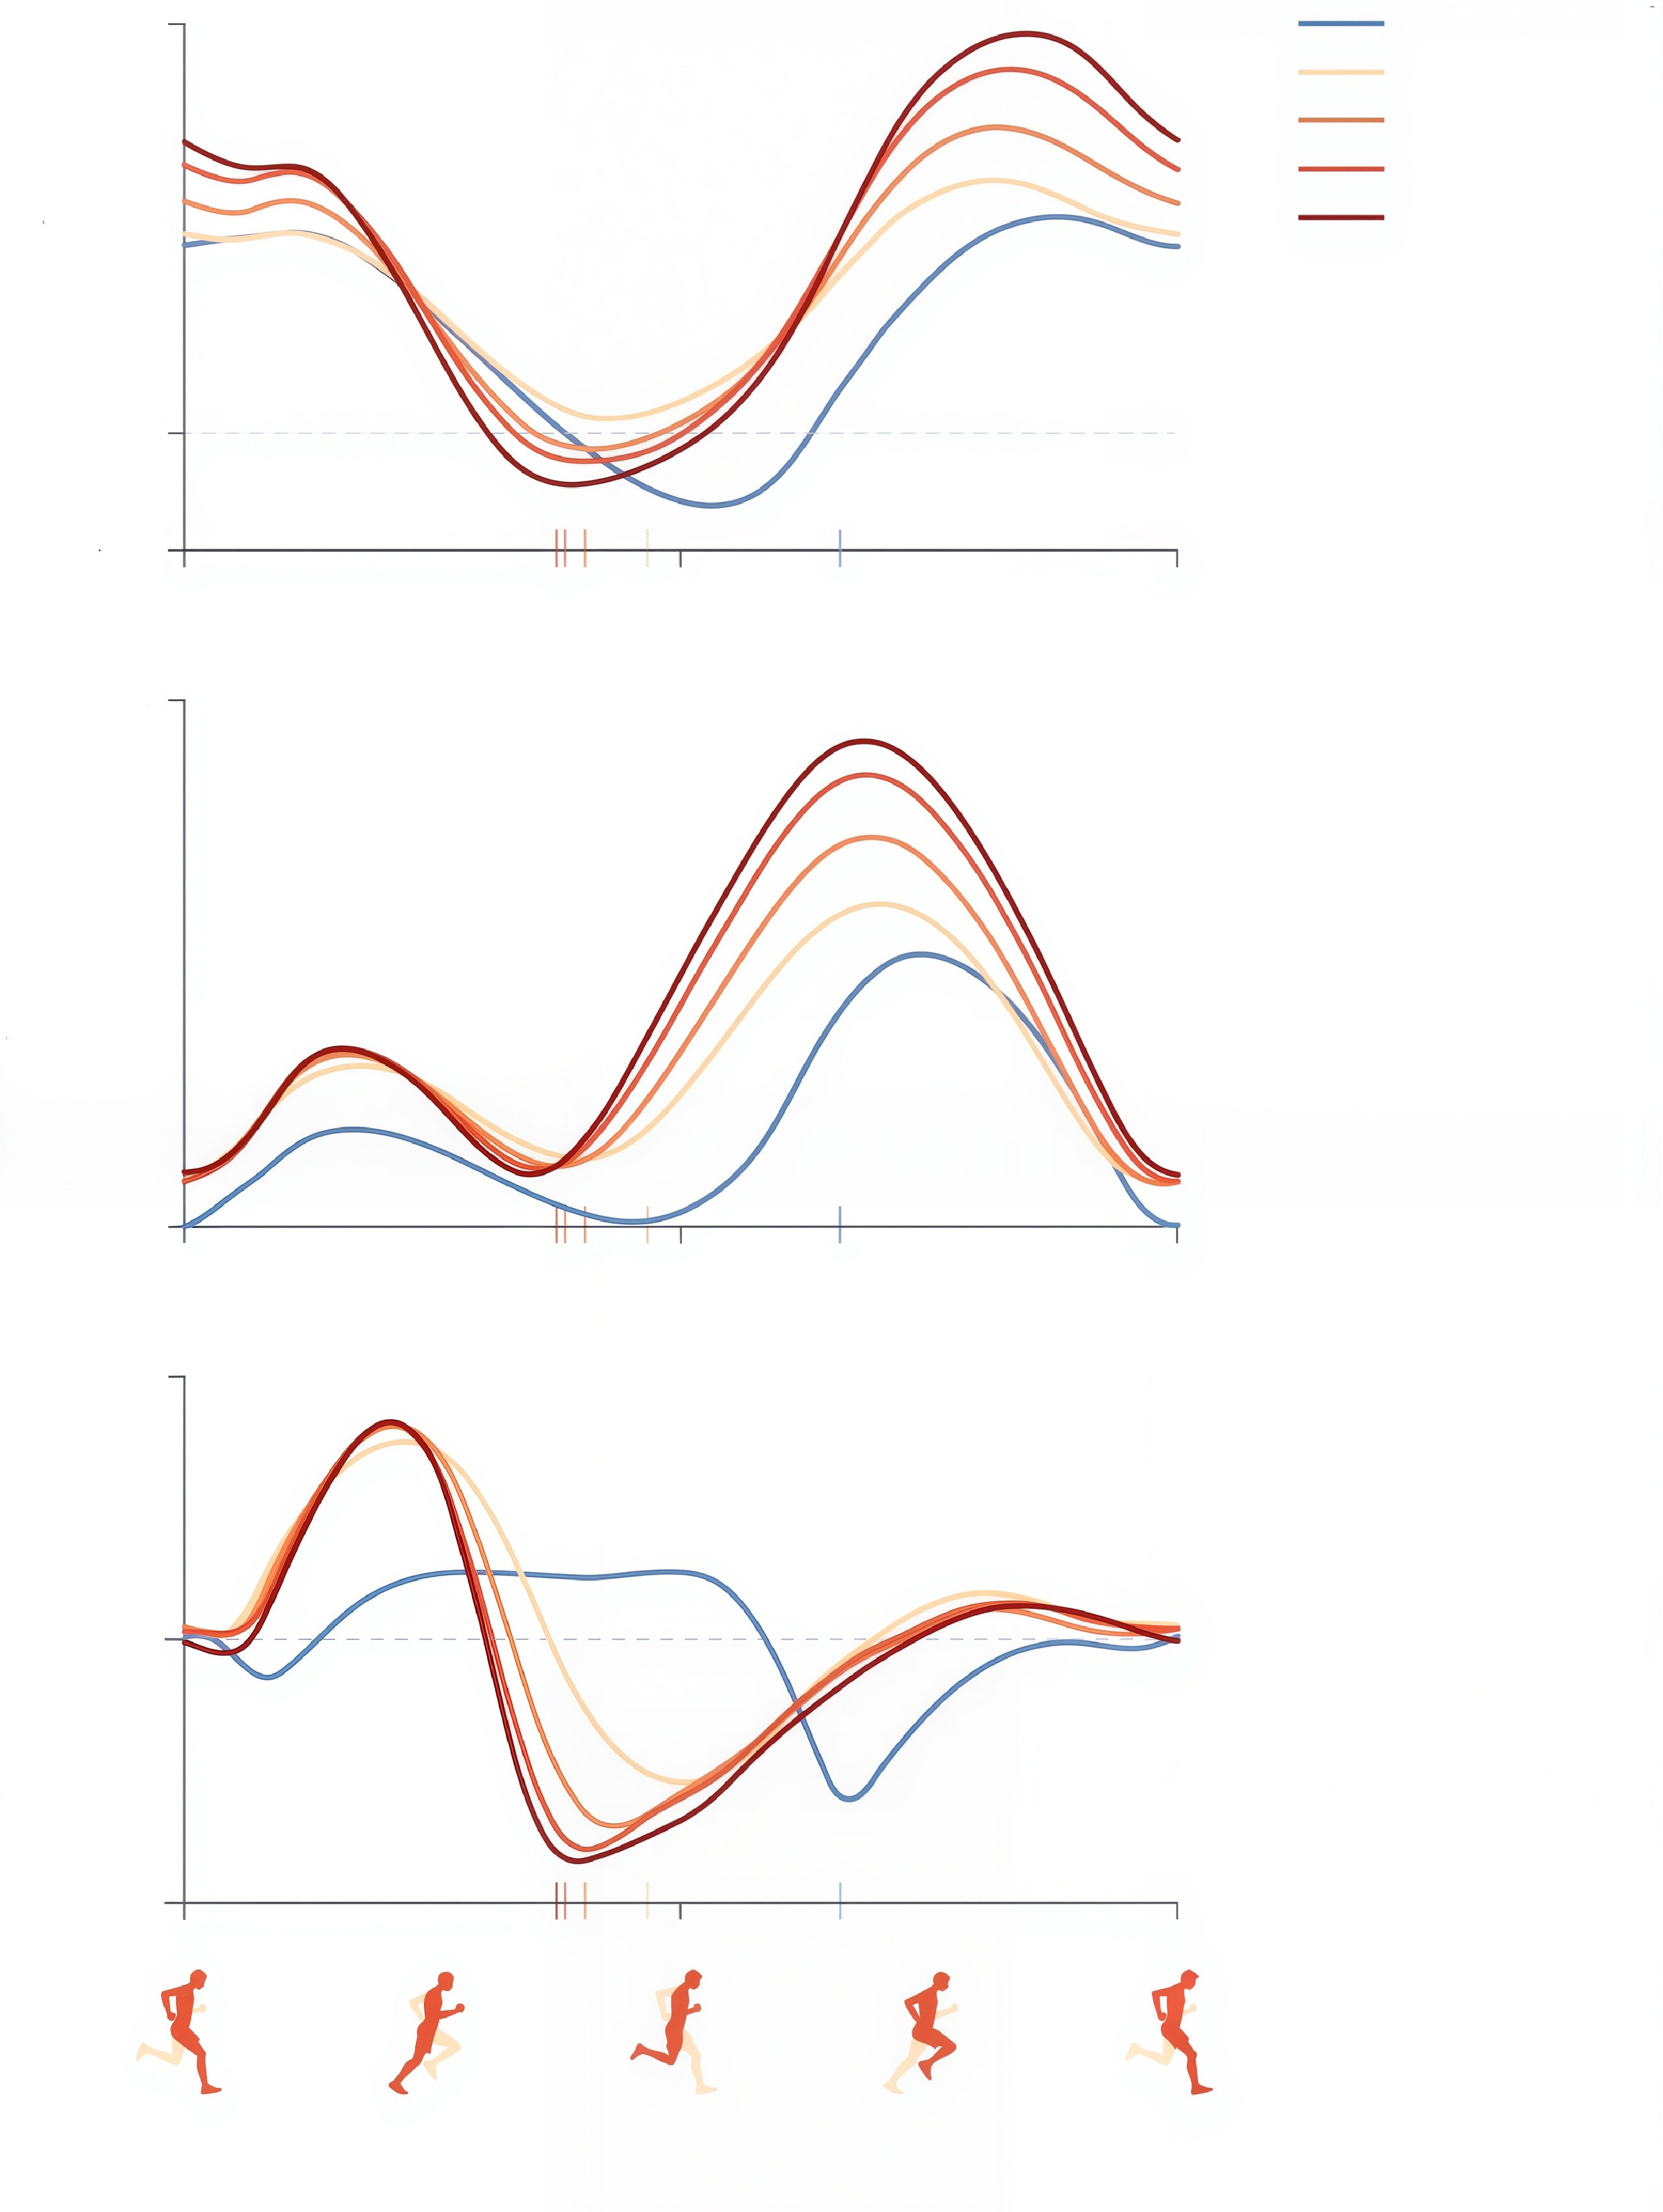
\includegraphics[width=1.0\linewidth]{chap3/3_20}
	\caption{以不同速度跑步时,步态周期内代表性关节运动。
		图~\ref{fig:2_19}~中以 1.5 米/秒的速度行走的样本可供参考。
		取 10 位受试者的平均值。
		横轴上的垂直线表示每种速度下的脚趾离地情况\cite{hamner2013muscle}。 \label{fig:3_20}}
\end{figure}


支撑期关节的运动有几个显著的特征。
髋部在足部触地时(步态周期的0\%)屈曲,并在支撑期持续伸展。
相比之下,膝部在足部触地时开始轻微屈曲,在支撑期的第一阶段屈曲,然后在支撑期的第二阶段伸展。
这种膝关节屈曲模式有助于支撑期腿部的压缩和伸展,从而导致肢体的弹簧状行为。
对于以脚跟着地的跑步者来说,踝关节在足部触地时处于中立位置;
踝关节在支撑期的第一阶段背屈,在第二阶段跖屈,与膝关节协同作用,产生腿部的弹簧状行为。


在摆动期,髋部屈曲以使肢体前移。
膝部在摆动的前半段屈曲,使足部离地;
在摆动的后半段伸展,为落地做准备。
踝部在站立结束时高度跖屈,在摆动期背屈回到中立位,为落地做准备。


\section{地面反作用力和跑步速度}

在低速跑步(例如 2 米/秒)时,地面反作用力的垂直分量在约 2 个体重时达到峰值(图~\ref{fig:3_21})。
随着速度的增加,垂直地面反作用力的峰值也会增加,在 5 米/秒时增加到超过 2.5 个体重,在更高的跑步速度下则高达 3 个体重。
速度的增加还会增加站立前半段向后施加的水平力,以及在站立后半段加速重心向前的水平力。
地面接触时间随着速度的增加而缩短,这可以通过步态周期中站立时间的减少来观察。


\begin{figure}[!htb]
	\centering
	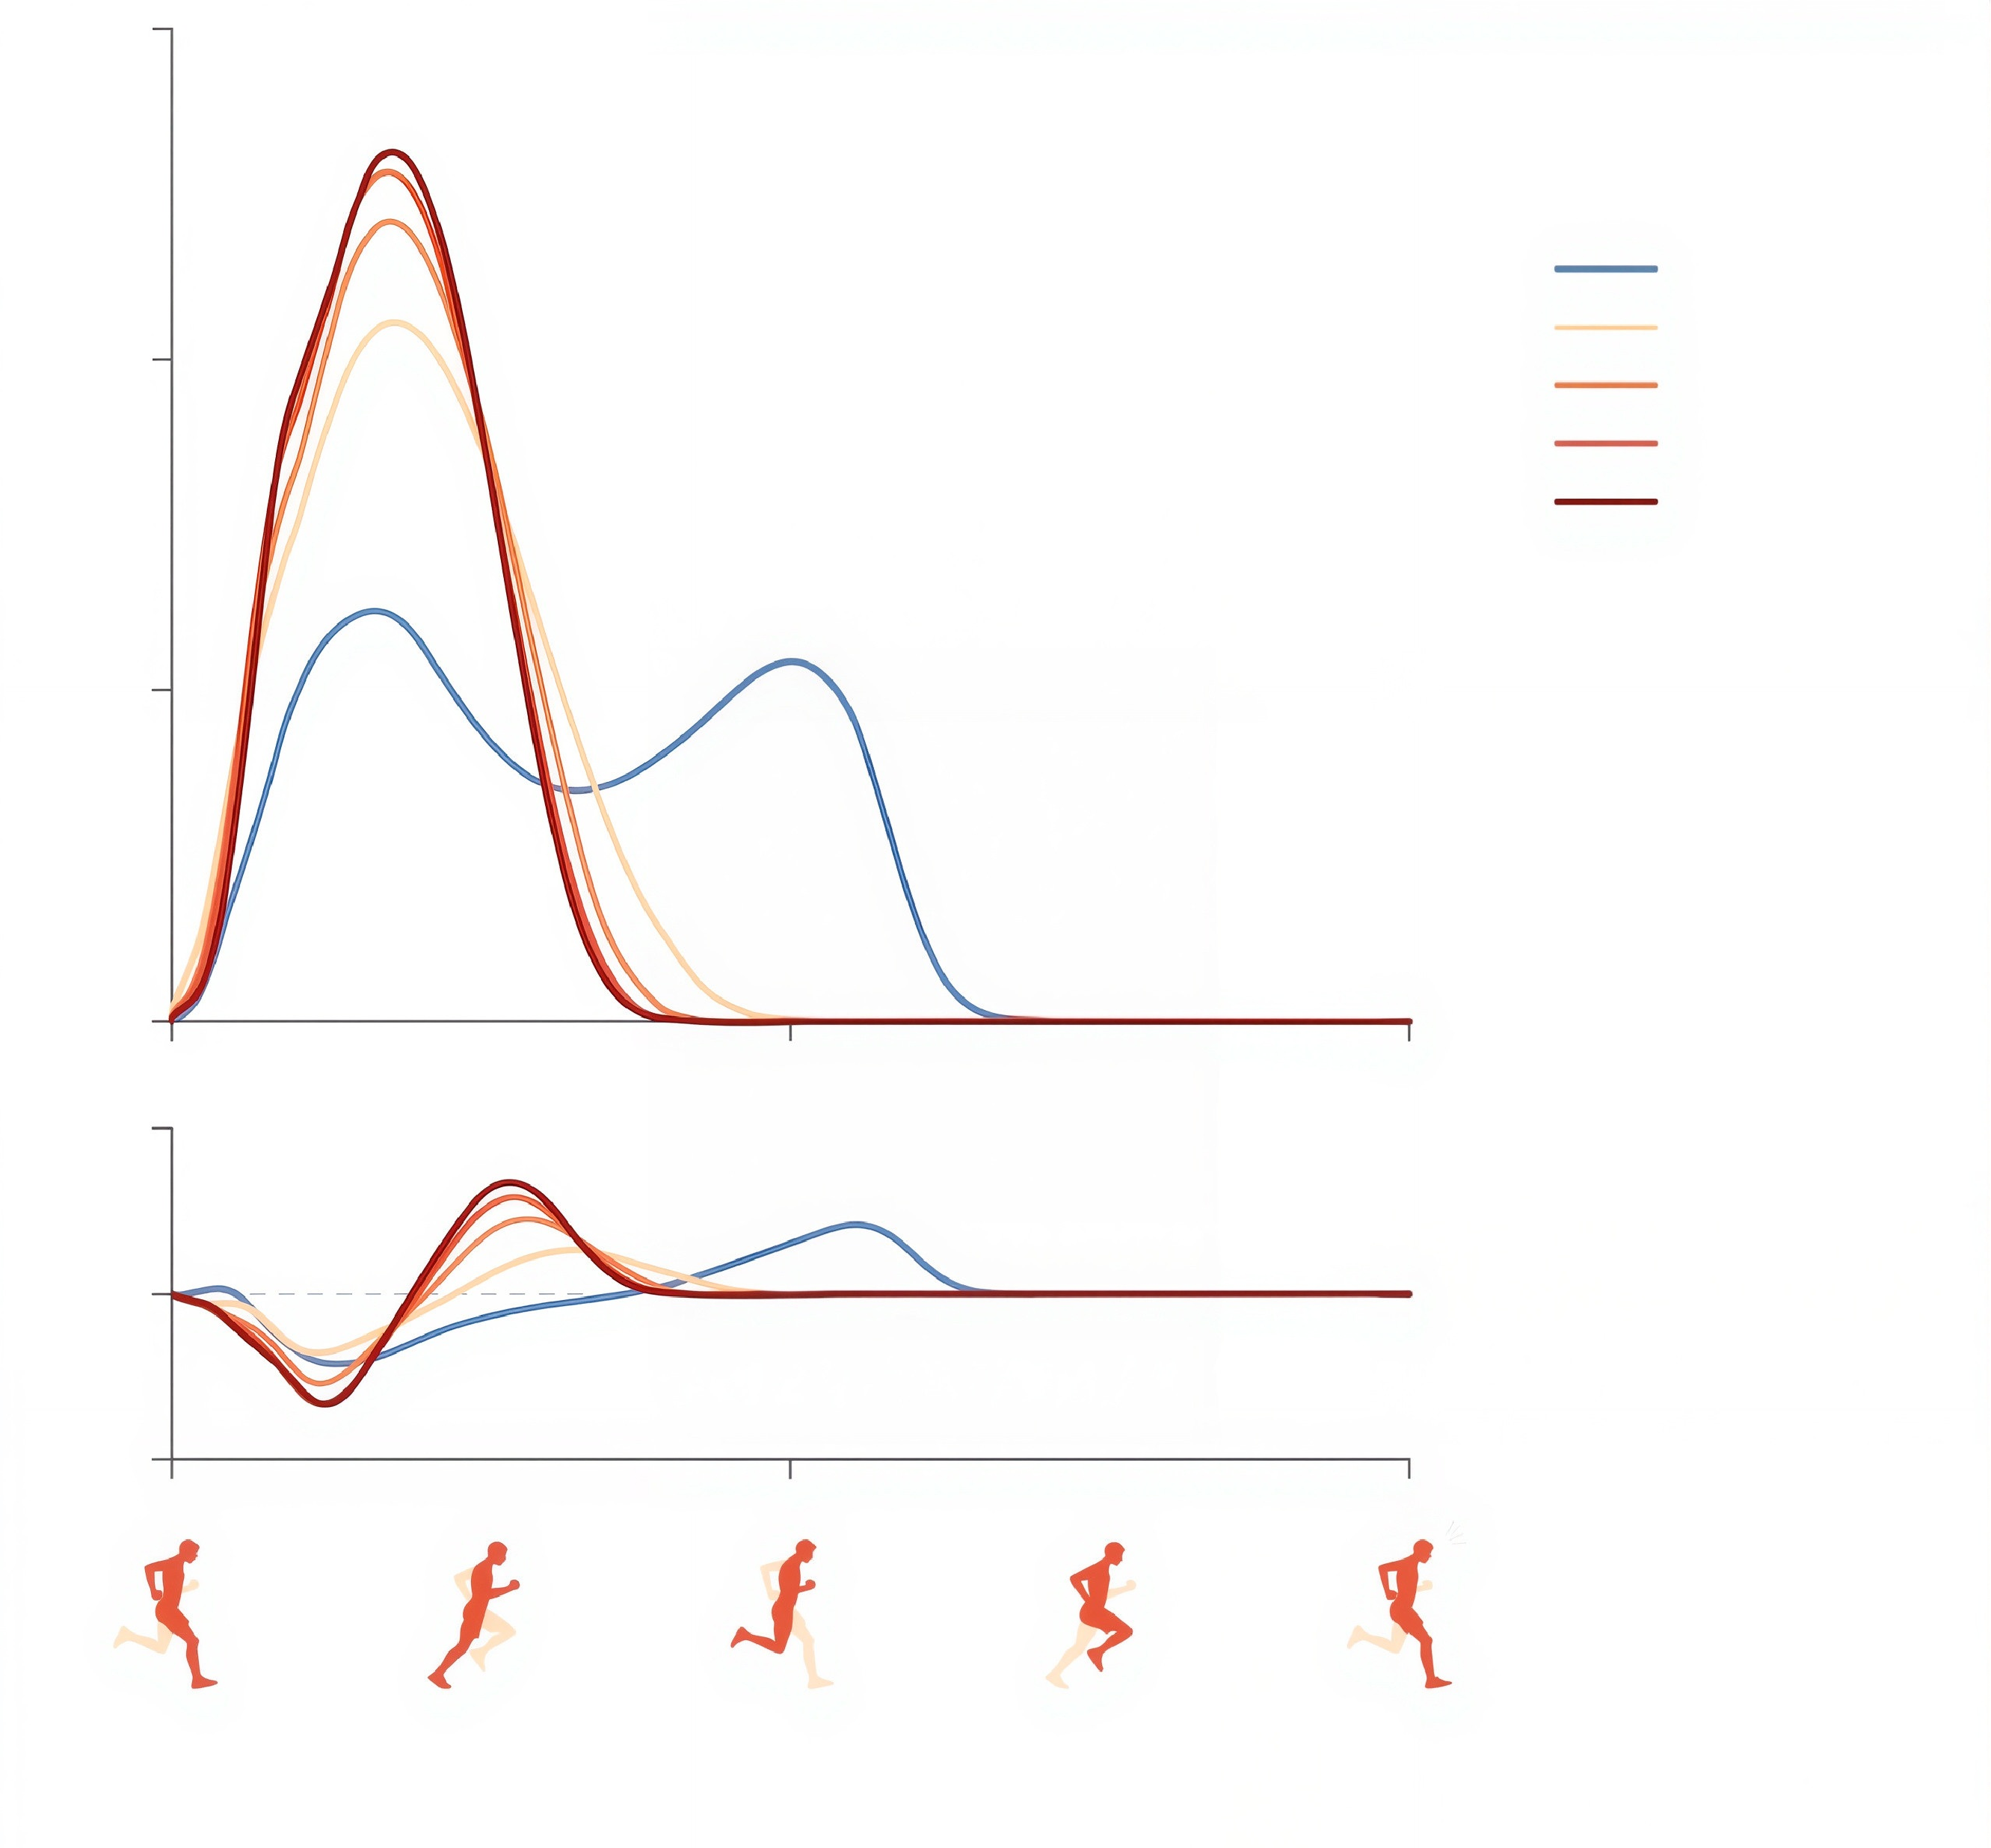
\includegraphics[width=1.0\linewidth]{chap3/3_21}
	\caption{以不同速度跑步时,步态周期内代表性地面反作用力。
		图~\ref{fig:2_20}~中以 1.5 米/秒的速度行走的步态供参考。
		已按体重标准化,并取 10 名受试者的平均值\cite{hamner2013muscle}。 \label{fig:3_21}}
\end{figure}


到目前为止,我们已经分析了高达 5 米/秒(相当于马拉松的快速配速)的稳态跑步,但人类最快的短跑运动员的速度可以达到这个速度的两倍以上。
Tim Dorn 及其同事研究了高速短跑,发现跑步者使用两种策略来提高速度\cite{dorn2012muscular}。
在 7 米/秒左右之前,跑步速度的提高主要通过产生更大的地面反作用力来推动身体向上和向前,从而增加步幅。
超过 7 米/秒后,地面反作用力不再增加,提高跑步速度的策略从增加步幅转变为增加步频,通过在腾空阶段更快速地移动腿部来实现。
我们将在第~\ref{chap:chap12}~章中看到肌肉是如何被运用来实现高速跑步的。


在关于行走和跑步的这两章中,我们运用简单的力学模型来阐述步态的一些基本特征,包括我们如何在行走中利用钟摆动力学,以及在跑步中利用弹性能来高效移动。
我们还详细研究了地面反作用力,因为这些记录可以反映施加在足部的力量以及重心如何加速。
我们尽可能地深入地阐述了这一点,而没有明确描述人类运动中至关重要的组成部分——肌肉。


正如我们上文所暗示的,正是肌肉和肌腱赋予了腿部类似弹簧的特性。
虽然我们可以测量地面反作用力,但如果不考虑肌肉骨骼系统的动力学,我们就无法确定是哪些肌肉力产生了这些反作用力。
一旦我们计算出肌肉力,就能估算出髋关节、膝关节或踝关节的负荷大小,从而开始了解关节损伤或设计人工关节。
在接下来的章节中,我们将探索肌肉的结构、功能和计算建模(第~\ref{chap:chap4}-\ref{chap:chap6}~章),然后介绍通过实验测量运动来估算关节运动和肌肉力的方法(第~\ref{chap:chap7}-\ref{chap:chap9}~章)。
之后,我们将在第~\ref{chap:chap10}-\ref{chap:chap12}~章中探索人类在行走和跑步过程中是如何协调肌肉的。










